\documentclass[a4paper]{article}	
\usepackage{graphicx} % Required for inserting images
\usepackage{amsmath}
\usepackage[]{geometry}
\usepackage{amssymb}
\usepackage{graphicx}
\usepackage{epstopdf}
\usepackage{inputenc}
\usepackage{geometry} 
\usepackage[pdfusetitle, colorlinks]{hyperref}
\usepackage{subcaption}
\usepackage[italian]{babel}
\usepackage{framed}
\usepackage{xcolor}
\usepackage{blindtext}
\usepackage{mathtools}
\usepackage{titlesec}
\usepackage{color,soul}
\usepackage{cancel}
\usepackage{tikz}
\usepackage{stmaryrd}
\usepackage{amsthm}
\usepackage{circledsteps}
\usepackage{pstricks}
\usepackage{comment}

\usepackage{mdframed} %pacchetto per leftbar non sfalzate fra di loro
\usetikzlibrary{shapes}



\begin{document}	
\newcommand{\mail}[3][blue]{\href{#2}{\color{#1}{#3}}}%



\newcommand\vertarrowbox[3][2ex]{%
	\begin{array}[t]{@{}c@{}} #2 \\
		\left\downarrow\vcenter{\hrule height #1}\right.\kern-\nulldelimiterspace\\
		\makebox[0pt]{\scriptsize#3}
	\end{array}%
}


\newmdenv[
topline=false,
bottomline=false,
rightline=false,
leftline=true,
linecolor=gray,
linewidth=2pt,
innerrightmargin=0pt,
skipabove=\baselineskip,
skipbelow=\baselineskip
]{exbar}

\newmdenv[
topline=false,
bottomline=false,
rightline=false,
leftline=true,
linecolor=black,
linewidth=2pt,
innerrightmargin=0pt,
skipabove=\baselineskip,
skipbelow=\baselineskip
]{dembar}

\newmdenv[
topline=false,
bottomline=false,
rightline=false,
leftline=true,
linecolor=red,
linewidth=2pt,
innerrightmargin=0pt,
skipabove=\baselineskip,
skipbelow=\baselineskip
]{attbar}


\everymath{\displaystyle}

\theoremstyle{definition}
\newtheorem{definition}{Definizione}[section]
\newtheorem{proposition}{Proposizione}[section]
\newtheorem{example}{Esempio}[section]

\theoremstyle{plain}
\newtheorem{theorem}{Teorema}[section]
\newtheorem{corollary}{Corollario}[theorem]
\newtheorem{lemma}[theorem]{Lemma}

\numberwithin{equation}{subsection}

\newcommand\distr
{\underset{\mbox{\tiny{triangolare}}}{\stackrel{\mbox{\tiny{disugualianza}}}{\leq}}}

\newcommand{\myarrow}[1][-45]{%
	\mathrel{%
		\text{$
			\begin{tikzpicture}[baseline = -0.5ex]
				\node[inner sep=0pt,outer sep=0pt,rotate = #1] (a) at (0,0)  {$\rightarrow{}$};
			\end{tikzpicture}
			$}%
	}%
}%

\makeatletter
\newcommand\mathcircled[1]{%
	\mathpalette\@mathcircled{#1}%
}
\newcommand\@mathcircled[2]{%
	\tikz[baseline=(math.base)] \node[draw,ellipse,inner sep=1pt] (math) {$\m@th#1#2$};%
}

\newcommand\inflim{\lim_{n \rightarrow +\infty}}

\newcommand\uppercomment[3]{
\mathcircled{#1}^{\color{blue}{\genfrac{}{}{0pt}{}{#2}{#3}}}
}

\newcommand\lowercomment[3]{
	\mathcircled{#1}_{\color{blue}{\genfrac{}{}{0pt}{}{#2}{#3}}}
}

\newcommand\undercomment[3]{
	\vertarrowbox{\mathcircled{#1}} {\color{blue}{$\genfrac{}{}{0pt}{}{#2}{#3}$}}
}


\makeatother


	
	\title{\Huge Analisi Matematica 2}
	\author{{\Large Emanuele Urso} \\
	{\small{\href{mailto:emanuele.urso@studenti.unipd.it}{\color{black}{emanuele.urso@studenti.unipd.it} }}}}
	\date{2022/2023}
	\maketitle
	
	\begin{figure}[!h]
		\centering
		\includegraphics[width=0.5\linewidth]{UniPdlogo.png}
	\end{figure}
	
	\vfill
	
	Questo libro è tratto dalle lezioni del canale M-Z della facoltà di fisica dell'università di Padova, tenute durante l'anno accademico 2023. Ci tengo a ringraziare \textbf{Giacomo Veglio} per aver contribuito al progetto fornendomi parte del materiale per la stesura di questo manuale.
	
	\vspace{10em}
	
	
	\begin{center}
		\rule{.9\textwidth}{0.4pt}%
	\end{center}
	
	\hypersetup{linkcolor=black}
	\tableofcontents   
	
\newpage

\section{Serie numeriche} 
\subsection{Introduzione}

\begin{gather*}
	\sin x = \sum_{k=0}^{\infty} (-1)^{k} \frac{x^{2k+1}}{(2k+1)!}
	\\
	\sin 4 = \sum_{k=0}^{\infty} (-1)^{k} \frac{4^{2k+1}}{(2k+1)!} = 
	4 - \frac{4^3}{3!} + \frac{4^5}{5!} - \frac{4^7}{7!} + \ldots 
	\\
	\sum_{k=1}^{\infty} \frac{1}{k} = 1 + \frac{1}{2} + \frac{1}{3} + \frac{1}{4} + \frac{1}{5} + \ldots = +\infty
	\\
	\sum_{k=1}^{5} \frac{1}{k} = 1 + \frac{1}{2} + \frac{1}{3} + \frac{1}{4} + \frac{1}{5} 
	\\
	\sum_{k=1}^{10} \frac{1}{k} = 1 + \frac{1}{2} + \frac{1}{3} + \ldots + \frac{1}{10}
	\\
	\sum_{k=1}^n \frac{1}{k} = 1 + \frac{1}{2} + \frac{1}{3} + \ldots + \frac{1}{n} \qquad n \geq 1 
	\\
	\sum_{k=1}^{\infty} \frac{1}{k} = \lim_{n\rightarrow\infty} \sum_{k=1}^{n} \frac{1}{k} 
\end{gather*}


\begin{definition} 
	Una serie a valori in $\mathbb{C}$ è una coppia $(\{a_n\}_{n \in \mathbb{N}}, \{S_n\}_{n\in\mathbb{N}})$ tale che $\{a_n\}_{n\in\mathbb{N}} \subseteq \mathbb{C}$ è una successione e $\{S_n\}_{n\in\mathbb{N}}$ è la successione delle ridotte.
	$S_n=\sum_{k=0}^{n} a_k$ si dice ridotta n-esima.
\end{definition}


\begin{exbar} 
	\begin{gather*}
		S_0=a_0 \qquad S_1=a_0+a_1 \qquad	S_2=a_0+a_1+a_2 \\
		S_3=a_0+a_1+a_2+a_3 \qquad \ldots \qquad S_n=a_0+a_1+\ldots+a_n
	\end{gather*}
\end{exbar}

La coppia $(\{a_n\}_{n \in \mathbb{N}}, \{S_n\}_{n\in\mathbb{N}})$ è identificata con $\sum_{k=0}^{\infty} a_k$

\begin{definition}
	Una serie $\sum_{k=0}^{\infty} a_k$ si dice:
	\begin{enumerate}
		\item \textbf{Convergente} se converge la successione delle ridotte, cioè se $\exists$ finito
		
		$\lim_{n\rightarrow+\infty} S_n = \lim_{n\rightarrow+\infty} \sum_{k=0}^{n} a_k$
		
		\item \textbf{Divergente} 
		\begin{enumerate}
			\item a $+\infty$ se $\lim_{n\rightarrow+\infty} S_n = +\infty$
			\item a $-\infty$ se $\lim_{n\rightarrow+\infty} S_n = -\infty$
			\item a $\infty$ se $\lim_{n\rightarrow+\infty} S_n = \infty$, cioè se $\lim_{n\rightarrow+\infty} |S_n| = +\infty$
		\end{enumerate}
		
		\item  \textbf{Irregolare o indeterminata} se $\lim_{n\rightarrow+\infty} S_n$ non esiste.
	\end{enumerate}
\end{definition}

\begin{exbar}
	$\sum_{k=0}^\infty (-1)^k \frac{4^{2k+1}}{(2k+1)!} = \lim_{n\rightarrow+\infty} \sum_{k=0}^n (-1)^k \frac{4^{2k+1}}{(2k+1)!} = \sin(4)$ è convergente;
	
	$\sum_{k=1}^\infty \frac{1}{k} = \lim_{n\rightarrow+\infty}\sum_{k=1}^n = +\infty$ è divergente. 
\end{exbar}

\begin{definition}
	Se la serie $\sum_{k=0}^{\infty} a_k$ converge, il $\lim_{n\rightarrow+\infty} S_n = \lim_{n\rightarrow+\infty} \sum_{k=0}^{n} a_k$ si dice somma della serie ed è indicato con $\sum_{k=0}^\infty a_k$
\end{definition}

\begin{proposition}
	\label{prop:serie complessa}
	Sia $\sum_{k=0}^\infty a_k$ una serie a termini complessi. Allora $\sum_{k=0}^\infty a_k$ converge $\iff$ convergono $\sum_{k=0}^\infty \mathrm{Re}(a_k)$ e $\sum_{k=0}^\infty \mathrm{Im}(a_k)$
\end{proposition}

\begin{exbar}
	$a_k = \alpha_k + i \beta_k$ \qquad $\alpha_k$, $\beta_k\in\mathbb{R}$ \qquad $\alpha_k = \mathrm{Re}(a_k)$, $\beta_k = \mathrm{Im}(a_k)$
	
	$\sum_{k=0}^\infty a_k$ converge $\iff$ convergono entrambe le serie a termini in $\mathbb{R}$ $\sum_{k=0}^\infty \alpha_k$ e $\sum_{k=0}^\infty \beta_k$.
\end{exbar}

Della serie è interessante studiare il carattere, cioè se convergono, divergono o sono irregolari.

\begin{dembar}
	\textbf{Dimostrazione} della \textbf{Proposizione \ref{prop:serie complessa}} 
	\begin{itemize}
		\item \textit{Condizione sufficiente $(\Rightarrow)$}: $\sum_{k=0}^\infty a_k$ converge $\Rightarrow \sum_{k=0}^\infty \alpha_k$ e $\sum_{k=0}^\infty \beta_k$ convergono. 
		
		Sia $S_a + iS_b$ la somma di $\sum_{k=0}^\infty a_k$, $S_a + iS_b = \lim_{n\rightarrow+\infty} \sum_{k=0}^n (\alpha_k + i\beta_k)$.
		
		Faccio vedere che $\lim_{n\rightarrow+\infty} \sum_{k=0}^n \alpha_k = S_a$ e $\lim_{n\rightarrow+\infty} \sum_{k=0}^n \beta_k = S_b$.
		
		$0 \leq \biggl|\sum_{k=0}^n \alpha_k - S_a \biggr| = \biggl|\mathrm{Re}(\sum_{k=0}^n a_k - (S_a + iS_b)) \biggr| \leq \biggl| \sum_{k=0}^n a_k - (S_a + iS_b) \biggr| \rightarrow 0$ per $n\rightarrow+\infty$
		
		Per il teorema del confronto $\lim_{n\rightarrow+\infty} \biggl| \sum_{k=0}^n \alpha_k -S_a \biggr| = 0 \iff \lim_{n\rightarrow+\infty} \sum_{k=0}^n \alpha_k = S_a$.
		
		In modo analogo si dimostra che $\lim_{n\rightarrow+\infty} \sum_{k=0}^n \beta_k = S_b$.
		
		\vspace{5pt}
		
		\item \textit{Condizione necessaria $(\Leftarrow)$}: 
		$\sum_{k=0}^\infty \alpha_k$ e $\sum_{k=0}^\infty \beta_k$ convergono $\Rightarrow$ $\sum_{k=0}^\infty a_k$ converge. 
		
		\begin{equation*}
			\lim_{n\rightarrow+\infty} \sum_{k=0}^n \alpha_k = S_a \in \mathbb{R} \qquad \lim_{n\rightarrow+\infty} \sum_{k=0}^n \beta_k = S_b \in \mathbb{R}
		\end{equation*}
		\begin{align*}
			0 \leq \biggl| \sum_{k=0}^n a_k - (S_a + iS_b) \biggr|
			&= \biggl| (\sum_{k=0}^n \alpha_k -S_a) + i(\sum_{k=0}^n \beta_k - S_b) \biggr| \\
			& \distr \biggl| \sum_{k=0}^n \alpha_k -S_a) \biggr| + \biggl| \sum_{k=0}^n \beta_k - S_b \biggr| \xrightarrow{n\rightarrow+\infty}  0 
		\end{align*}
		
		e si conclude con il teorema del confronto. $\square$
	\end{itemize}
\end{dembar}


\subsubsection{Paradosso di Zenone} 
\begin{figure}[!h]
	\centering
	\includegraphics[width=0.7\linewidth]{serie_numeriche/zenone.png}
	\caption{Paradosso di Zenone}
	\label{fig:zenone}
\end{figure}

A Achille, T tartaruga, $v_A>v_T$ 

\begin{align*}
\centering
L_0 & \qquad t_0 = \frac{L_0}{v_A} 
\\
L_1=t_0\cdot v_T & \qquad t_1=\frac{L_1}{v_A} = t_0\frac{v_T}{v_A}
\\
L_2=t_1\cdot v_T & \qquad t_2=\frac{L_2}{v_A} = t_1 \frac{v_T}{v_A} = t_0 \biggl( \frac{v_T}{v_A} \biggr) ^2 
\\
L_3=t_2\cdot v_T & \qquad t_3=\frac{L_3}{v_A} =  t_0 \biggl( \frac{v_T}{v_A} \biggr) ^3
\end{align*}
Quanto tempo impiega Achille a raggiungere la tartaruga?

\newcommand\zenone{\stackrel{\mbox{\tiny{$v_T<v_A$}}}{=}}

\begin{align*}
	T   &= t_0 + t_1 + t_2 + \ldots = t_0 \biggl(1 + \frac{v_T}{v_A} + \biggl(\frac{v_T}{v_A}\biggr)^2 + \ldots + \biggl(\frac{v_T}{v_A}\biggr)^n + \ldots \biggr)	= t_0 \sum_{k=0}^\infty \biggl(\frac{v_T}{v_A}\biggr)^k = \\
	&\zenone t_0 \frac{1}{1-\frac{v_T}{v_A}} = \frac{\frac{L_0}{v_A}}{1-\frac{v_T}{v_A}}
\end{align*}

\subsubsection{Serie geometrica} di ragione r, con $r\in\mathbb{C}$

\begin{equation*}
	\sum_{k=0}^\infty r^k = r^0 + r^1 + r^2 + \ldots
\end{equation*}

\begin{itemize}
	\item $r=1$
	\begin{align*}
		\sum_{k=0}^\infty 1^k
		&= \lim_{n} \sum_{k=0}^n 1^k = \lim_{n} \underbrace{(1 + 1 + \ldots +1)}_\text{n+1 volte} = \\
		&=\lim_{n} (n+1) = +\infty
	\end{align*}
	
	\item $r\neq1$ \qquad Procuriamoci un'espressione della ridotta n-esima, cioè 
	\begin{equation*}
		S_n = \sum_{k=0}^n r^k = 1 + r + r^2 + \ldots + r^n
	\end{equation*}
	
	\begin{gather*}
		\begin{cases*}
			S_{n+1} = \sum_{k=0}^{n+1} r^k = \underbrace{1 + r + r^2 + \ldots + r^n}_\text{$S_n$} + r^{n+1} = S_n + r^{n+1} \\
			S_{n+1} = 1 + \underbrace{r + r^2 +r^3 + \ldots + r^n + r^{n+1}}_\text{raccolgo r a fattore comune} = 1 + r(1 + r + r^2 + \ldots + r^n) = 1 + rS_n
		\end{cases*}  \Rightarrow
		\\
		\Rightarrow S_n + r^{n+1} = 1 + rS_n
	\end{gather*}
	

	
	\begin{equation}
		S_n = \frac{1 - r^{n+1}}{1-r}
	\end{equation}
\end{itemize}

\begin{exbar}
	Per Achille e la Tartaruga $r=\frac{v_T}{v_A}$.
\end{exbar}

\begin{attbar}
	$\lim_{n} S_n = \lim_{n} \frac{1-r^{n+1}}{1-r} \exists$ finito e vale in tal caso $\frac{1}{1-r} \iff |r|<1$
\end{attbar}

\begin{attbar}
	La serie geometrica di ragione $r$, $\sum_{k=0}^\infty r^k$ converge $\iff |r|<1$ e in tal caso la sua somma vale $\frac{1}{1-r}$.
\end{attbar}

\begin{exbar}
	\begin{example} Dimostriamo che $0.\bar{9} = 1$
		\begin{align*}
			0.\bar{9} 
			&= \sum_{k=1}^\infty \frac{9}{10^k} = \lim_{n\rightarrow+\infty} \sum_{k=1}^n \frac{9}{10^k} = 9 \lim_{n\rightarrow+\infty} \sum_{k=1}^n \frac{1}{10^k} = 9 \lim_{n\rightarrow+\infty} \biggl( \sum_{k=0}^n \frac{1}{10^k} - \frac{1}{10^0} \biggr) = \\
			&= 9 \biggl( \sum_{k=0}^\infty \biggl(\frac{1}{10} \biggr)^k - 1 \biggr) = 9 \biggl( \frac{1}{1-\frac{1}{10}} -1 \biggr) = 9 \biggl( \frac{10}{9} -1 \biggr) = \\
			&=1
		\end{align*}	
	\end{example}
\end{exbar}

\subsubsection{Serie telescopiche}
\begin{equation*}
	\sum_{k=0}^\infty [f(k+1) - f(k)] \qquad f:\mathbb{N}\rightarrow\mathbb{C}
\end{equation*}


Studiamo il carattere. Procuriamoci, se possibile, l'espressione di una ridotta n-esima
\begin{align*}
	S_n &= \sum_{k=0}^n [f(k+1)-f(k)] = \\
	&= \overbrace{\cancel{f(1)}-f(0)}^{k=0} + \overbrace{\cancel{f(2)}-\cancel{f(1)}}^{k=1} + \overbrace{\cancel{f(3)}-\cancel{f(2)}}^{k=2} +  \overbrace{\cancel{f(4)}-\cancel{f(3)}}^{k=3} + \ldots + \overbrace{f(n+1)-\cancel{f(n)}}^{k=n} = \\
	&= f(n+1) -f(0)
\end{align*}
\begin{attbar}
	$\lim_{n}S_n = \lim_{n}[f(n+1)-f(0)]$ esiste $\iff$ esiste $\lim_{n} f(n)$.
	
	La serie converge $\iff$ $\lim_{n} f(n)$ esiste finito e in tal caso la somma della serie è 
	\begin{equation*}
			\sum_{k=0}^\infty [f(k+1)-f(k)] = \lim_{n\rightarrow+\infty} f(n)-f(0)
	\end{equation*}

\end{attbar}

\begin{exbar}
	\begin{example} (serie di Mengoli)
		\begin{align*}
			\sum_{k=1}^\infty \frac{1}{k(k+1)} 
			&= \sum_{k=1}^\infty \biggl( \frac{1}{k} -\frac{1}{k+1} \biggr) \\
			&= -\sum_{k=1}^\infty \biggl[\frac{1}{k+1} - \frac{1}{k}\biggr] & \mathrm{dove} \, \frac{1}{k}=f(k) \\
			&= -\lim_{n}[f(n)-f(1)] = f(1) = \\
			&= 1
		\end{align*}
	\end{example}
\end{exbar}

\subsubsection{Formula di Eulero} 

\begin{gather*}
	e^{i\theta} = \cos(\theta) + i \sin(\theta) 
	\\	
	e^{in\theta} = \cos(n\theta) + i\sin(n\theta)
	\\	
	\sum_{n=0}^\infty [\cos(n\theta)+i\sin(n\theta)] = \sum_{n=0}^\infty e^{in\theta} =  \sum_{n=0}^\infty (e^{i\theta})^n
\end{gather*}
Non converge, perché è una serie geometrica di ragione $e^{i\theta}$ e $|e^{i\theta}| = 1$.

Se $\theta = 0, 2\pi$:
\begin{itemize}
	\item $\sum_{n=0}^\infty \cos(n\theta) = \sum_{n=0}^\infty 1 = +\infty$
	\item $\sum_{n=0}^\infty \sin(n\theta) = \sum_{n=0}^\infty 0 = 0$
\end{itemize}

Se $\theta \neq 0, 2\pi$:
\begin{itemize}
	\item $\sum_{k=0}^n \cos(k\theta) = \mathrm{Re} \bigg(\sum_{k=0}^n (e^{i\theta})^k \bigg) = \mathrm{Re} \bigg( \frac{1-e^{i\theta(n+1)}}{1-e^{i\theta}} \bigg)$
	\item $\sum_{k=0}^n \sin(k\theta) = \mathrm{Im} \bigg(\sum_{k=0}^n (e^{i\theta})^k \bigg) = \mathrm{Im} \bigg( \frac{1-e^{i\theta(n+1)}}{1-e^{i\theta}} \bigg)$
\end{itemize}

\begin{align*}
	& \qquad \frac{1-e^{i\theta(n+1)}}{1-e^{i\theta}} \\
	&= \frac{1 - \cos[(n+1)\theta] - i \sin[(n+1)\theta]}{1-\cos\theta - i \sin\theta} \\
	&= \frac{1 - \cos[(n+1)\theta] - i\sin[(n+1)\theta]}{|1-\cos\theta-i\sin\theta|^2} \cdot (1 - \cos\theta + i\sin\theta) \\
	&= \frac{1}{2(1-\cos\theta)} \cdot \{1 - \cos[(n+1)\theta] - i\sin[(n+1)\theta]\} \cdot (1 - \cos\theta + i\sin\theta)= \\
	&= \frac{1}{2(1-\cos\theta)} \cdot \{ 1 - \cos\theta - \cos[(n+1)\theta] + \cos\theta\cos[(n+1)\theta] + \sin\theta\sin[(n+1)\theta] + \\
	& \quad + i[\sin\theta-\cos[(n+1)\theta]\sin\theta - \sin[(n+1)\theta] + \sin[(n+1)\theta] \cos\theta ] \}
\end{align*}

Separiamo parte reale e immaginaria e raccogliamo:
\begin{gather*}
	\sum_{k=0}^n \cos(k\theta) =  \frac{1}{2(1-\cos\theta)} \cdot [(1-\cos\theta)(1-\cos((n+1)\theta)) + \sin\theta\sin((n+1)\theta)]
	\\
	\sum_{k=0}^n \sin(k\theta) =  \frac{1}{2(1-\cos\theta)} \cdot [\sin\theta(1-\cos((n+1)\theta)) - \sin((n+1)\theta)(1-\cos\theta)]
\end{gather*}	
	
	
\subsection{Studio del carattere di una serie}
\begin{theorem}
	\label{th:termine generale}
	$\{a_k \}_{k\in\mathbb{N}} \subseteq \mathbb{C}$ $($oppure $\mathbb{R})$. Se $\sum_{k=0}^\infty a_k$ converge, allora $\lim_{k\rightarrow+\infty} a_k = 0$.
\end{theorem}
Se una serie è convergente il suo termine generale è infinitesimo.

\begin{exbar}
	\begin{example} (serie armonica)
		
		\textbf{Non è vero} che $\lim_{k\rightarrow+\infty} a_k = 0 \Rightarrow \sum_{k=0}^\infty a_k$ converge.
		
		$\sum_{k=1}^\infty \frac{1}{k}$ serie armonica diverge, ma $\lim_{k\rightarrow+\infty}\frac{1}{k} = 0$.
		
		Prendiamo $x$ compresa tra due numeri interi $k$ e $k+1$, con $k\geq 1$.
		\begin{gather*}
			k\leq x \leq k+1
			\\
			\frac{1}{k+1} \leq \colorbox{yellow}{\parbox{1.1cm}{$\frac{1}{x} \leq \frac{1}{k}$}}
			\\
			\int_{k}^{k+1} \frac{1}{x} \mathrm{d}x \leq \int_{k}^{k+1} \frac{1}{k} \mathrm{d}x = \frac{1}{k}
			\\
			\frac{1}{k} \geq \int_{k}^{k+1} \frac{1}{x} \mathrm{d}x = \ln(k+1) -\ln(k)
			\\
			\sum_{k=1}^n \frac{1}{k} \geq \sum_{k=1}^n [\ln(k+1)-\ln(k)] = \ln(n+1)-\ln(1) = \ln(n+1) 
		\end{gather*}
		
		Per il teorema del confronto $\lim_{n}\sum_{k=0}^n \frac{1}{k} \geq \lim_{n} \ln(n+1) = +\infty \Rightarrow \sum_{k=1}^\infty \frac{1}{k} = +\infty$.
	\end{example}
\end{exbar}

\begin{attbar}
	Il \textbf{Teorema \ref{th:termine generale}} si può rileggere: se $\lim_{k\rightarrow+\infty} a_k \neq 0 \Rightarrow \sum_{k=0}^\infty a_k$ non converge.
\end{attbar}

Riprendendo l'esempio del paragrafo precedente vediamo che i termini generale di $\sin(k\theta)$ e $\cos(k\theta)$ non esistono: $\lim_{k\rightarrow+\infty} \cos(k\theta)$ non esiste se $\theta \neq \frac{\pi}{2}, \frac{3\pi}{2}$ e $\lim_{k\rightarrow+\infty} \sin(k\theta)$ non esiste se $\theta\neq 0, 2\pi$.

\begin{dembar}
	\textbf{Dimostrazione} del \textbf{Teorema \ref{th:termine generale}} 
	
	Sappiamo che $\sum_{k=0}^\infty a_k$ converge.
	
	\begin{gather*}
		S_n = \sum_{k=0}^n a_k \qquad S_{n-1} = \sum_{k=0}^{n-1} a_k
		\\
		S_n - S_{n-1} = \sum_{k=0}^n a_k - \sum_{k=0}^{n-1} a_k = a_n + \sum_{k=0}^{n-1} a_k - \sum_{k=0}^{n-1} a_k = a_n
		\\
		\lim_{n} a_n = \lim_{n} (\vertarrowbox{S_n}{$S$} - \vertarrowbox{S_{n-1}}{$S$}) = 0 
	\end{gather*}
	
	$S\in\mathbb{C}$ somma della serie. $\square$
\end{dembar}

\begin{proposition}
	\label{prop:somma convergenti}
	Siano $\sum_{n=0}^\infty a_n$ e $\sum_{n=0}^\infty b_n$ serie convergenti di somma $S_a$ ed $S_b$ rispettivamente. Allora $\sum_{n=0}^\infty (a_n + b_n)$ converge e la sua somma è $S_a+S_b$
\end{proposition}

\begin{dembar}
	\textbf{Dimostrazione} della \textbf{Proposizione \ref{prop:somma convergenti}}
	
	\begin{equation*}
		\sum_{k=0}^n (a_k + b_k) = \vertarrowbox{\sum_{k=0}^\infty a_k}{$S_a$} + \vertarrowbox{\sum_{k=0}^\infty b_k}{$S_b$} \xrightarrow{n\rightarrow+\infty} S_a + S_b \quad \square 
	\end{equation*}
	
\end{dembar}

\begin{proposition}
	\label{prop:prodotto convergente}
	Sia $\sum_{k=0}^\infty a_k$ serie convergente di somma S e sia $c\in\mathbb{C}$. Allora $\sum_{k=0}^\infty (c \cdot a_k)$ converge e la sua somma è $c \cdot S$
\end{proposition}

\begin{dembar}
	\textbf{Dimostrazione} della \textbf{Proposizione \ref{prop:prodotto convergente}}
	\begin{equation*}
		\sum_{k=0}^n (c\cdot a_k) = c\vertarrowbox{\sum_{k=0}^n a_k}{$S$} \xrightarrow{n\rightarrow+\infty} c\cdot S \quad \square
	\end{equation*}

\end{dembar}

\begin{proposition}
	\label{prop:stesso carattere}
	Sia data la serie $\sum_{k=0}^\infty a_k$ e sia $n_0\in\mathbb{N}$, $n_0\geq1$. Allora $\sum_{k=0}^\infty a_k$ e $\sum_{k=n_0}^\infty a_k$ hanno lo stesso carattere.
\end{proposition}

\begin{exbar}
	$\sum_{k=1}^\infty \frac{1}{k}$ e $\sum_{k=10^{10}}^\infty \frac{1}{k}$ hanno lo stesso carattere, quindi $\sum_{k=10^{10}}^\infty \frac{1}{k} = +\infty$.
\end{exbar}

\begin{attbar}
	Il carattere di una serie dipende solo dalla coda della successione dei suoi termini.
\end{attbar}

\begin{dembar}
	\textbf{Dimostrazione} della \textbf{Proposizione \ref{prop:stesso carattere}}
	
	Sia $n_0<n$ e $\sum_{k=0}^n a_k = \sum_{k=0}^{n_0-1} a_k + \sum_{k=n_0}^n a_k$
	
	$\lim_{n} \sum_{k=0}^n a_k$ esiste $\iff \exists \lim_{n\rightarrow+\infty} \sum_{k=n_0}^n a_k$ per la \textbf{Proposizione \ref{prop:somma convergenti}} e in tal caso 
	
	$\lim_{n} \sum_{k=0}^n a_k = \bigg(\lim_{n} \sum_{k=n_0}^n a_k \bigg) + \bigg(\sum_{k=0}^{n_0-1}a_k\bigg). \quad \square$
\end{dembar}

\begin{definition}
	Sia $\{a_n\}_{n\in\mathbb{N}}$ successione in $\mathbb{R}$ o in $\mathbb{C}$. Allora $\{a_n\}_{n\in\mathbb{N}}$ si dice di Cauchy se $\forall \; \varepsilon > 0 \; \exists \; N>0 \mid \forall \; n>N$ e $p\geq0$ \quad $\mid a_{n+p} - a_n \mid < \varepsilon$.
\end{definition}

\begin{theorem} (criterio di Cauchy per le successioni)
	Sia $\{a_n\}_{n\in\mathbb{N}}$ successione in $\mathbb{R}$ o in $\mathbb{C}$. Allora $\{a_n\}_{n\in\mathbb{N}}$ è convergente $\iff$ è di Cauchy
\end{theorem}

\begin{theorem} (criterio di Cauchy per le serie)
	\label{th:Cauchy serie}
	Sia data una serie $\sum_{k=0}^\infty a_k$ in $\mathbb{R}$ o in $\mathbb{C}$. Allora la serie converge $\iff \forall \; \varepsilon > 0 \; \exists \; N>0 \; \mid$ se $n>N$ e $p\geq0$ \quad $\biggl| \sum_{k=n}^{n+p} a_k \biggr| < \varepsilon$.
\end{theorem}

{\noindent Si ricava dal criterio di Cauchy per le successioni osservando che $\sum_{k=n}^{n+p} a_k = S_{n+p} - S_{n-1}$ \par}

\begin{proposition}
	\label{prop:no indeterminata}
	Sia $\sum_{k=0}^\infty a_k$ serie a termini definitivamente non negativi $\mathrm{(} \exists \; N>0 \; | \;$ \\ %riq malf
	$a_k\geq 0 \quad \forall \; k>N \mathrm{)}$. Allora la serie converge o diverge, non può essere indeterminata. 
\end{proposition}

\begin{dembar}
	\textbf{Dimostrazione} della \textbf{Proposizione \ref{prop:no indeterminata}}
	
	Per semplicità assumiamo $a_k \geq 0 \; \forall \; k\in\mathbb{N}$. Devo far vedere che, se $\{S_n \}_{n\in\mathbb{N}}$ è la successione delle ridotte, questa fa limite finito o infinito.
	\begin{equation*}
		S_{n+1} = \sum_{k=0}^{n+1} a_k = a_{n+1} + \sum_{k=0}^n = \vertarrowbox{a_{n+1}}{$\geq 0$} + S_n \geq S_n
	\end{equation*}
	
	$\{S_n \}_{n\in\mathbb{N}}$ è crescente e quindi fa limite finito o a $+\infty$. \quad $\square$
\end{dembar}

\begin{theorem}
	\label{th:convergenza assoluta}
	Sia data la serie $\sum_{k=0}^\infty a_k$ e si supponga che $\sum_{k=0}^\infty |a_k|$ converga (si dice che $\sum_{k=0}^\infty a_k$ converge assolutamente). Allora anche $\sum_{k=0}^\infty a_k$ converge e in tal caso $\bigg| \sum_{k=0}^\infty a_k \biggr| \leq \sum_{k=0}^\infty |a_k|$.
\end{theorem}

\begin{dembar}
	\textbf{Dimostrazione} del \textbf{Teorema \ref{th:Cauchy serie}}
	
	Siccome $\sum_{k=0}^\infty |a_k|$ converge, $\forall \; \varepsilon>0 \; \exists \; N>0 \; | $ se $n>N$ e $p\geq 0$ \quad $\sum_{k=n}^{n+p} |a_k| < \varepsilon$
	
	$\bigg| \sum_{k=n}^{n+p} a_k \bigg| \distr \sum_{k=n}^{n+p} |a_k| < \varepsilon$ se $n>N$ e $p\geq0 \Rightarrow$ la serie soddisfa la condizione di Cauchy e quindi converge.
	
	In tal caso 
	\begin{align*}
		\bigg| \sum_{k=0}^\infty a_k \bigg|
		& \quad = \bigg|\lim_{n\rightarrow+\infty} \sum_{k=0}^n a_k \bigg| = \lim_{n\rightarrow+\infty} \bigg| \sum_{k=0}^n a_k \bigg| \\
		&\distr \lim_{n\rightarrow+\infty} \sum |a_k| = \sum_{k=0}^\infty |a_k|. \quad \square
	\end{align*}
\end{dembar}

\begin{definition}
	Una serie si dice semplicemente convergente se converge, ma non necessariamente converge la serie dei moduli.
\end{definition}

\begin{attbar}
	Il \textbf{Teorema \ref{th:convergenza assoluta}} non si può invertire. Una serie potrebbe convergere semplicemente, ma non convergere assolutamente.  
\end{attbar}

\begin{exbar}
	$\sum_{k=1}^\infty \frac{(-1)^k}{k}$ converge, ma $\sum_{k=1}^\infty \bigg| \frac{(-1)^k}{k} \bigg| = \sum_{k=1}^\infty \frac{1}{k}$ è divergente.
\end{exbar}

\subsection{Criteri di convergenza di serie a termini non negativi}
\subsubsection{Criterio del confronto}
\begin{theorem} (criterio del confronto) 
	\label{th:criterio del confronto}
	
	$\{a_k \}_{k\in\mathbb{N}}$, $\{b_k \}_{k\in\mathbb{N}}$ successioni a termini definitivamente non negativi tali che $0\leq a_k \leq b_k$ definitivamente per $k\rightarrow+\infty$.
	
	\begin{enumerate}
		\item Se $\sum_{k=0}^\infty b_k$ converge, allora $\sum_{k=0}^\infty a_k$ converge;
		\item Se $\sum_{k=0}^\infty a_k$ diverge, allora $\sum_{k=0}^\infty b_k$ diverge.
	\end{enumerate}
\end{theorem}

\begin{dembar}
	\textbf{Dimostrazione} del \textbf{Teorema \ref{th:criterio del confronto}}
	
	Definiamo $S_n^b = \sum_{k=0}^n b_k, \; S_n^a = \sum_{k=0}^n a_k$ e per semplicità assumiamo che $a_k \leq b_k \; \forall \; k\geq 0$.
	
	$\lim_{n} S_n^b$ e $\lim_{n} S_n^a$ esistono perché le serie sono a termini definitivamente non negativi. 
	
	Se $\sum_{k=0}^\infty b_k$ converge $\Rightarrow \lim_{n} S_n^b = S^b < +\infty$ 
	
	$a_k \leq b_k \; \forall \; k \Rightarrow S_n^a \leq S_n^b \; \forall \; n$
	
	$\lim_{n} S_n^a \leq \lim_{n} S_n^b < +\infty \Rightarrow \lim_{n} S_n^a$ esiste $\Rightarrow \sum_{k=0}^\infty a_k$ converge.
	
	Se $\sum_{k=0}^\infty a_k$ diverge $\Rightarrow \lim_{n} S_n^a = +\infty$ e $S_n^b \geq S_n^a \; \forall \; n$
	
	$\lim_{n} S_n^b = +\infty$ per il teorema del confronto $\Rightarrow \sum_{k=0}^\infty b_k$ diverge. $\square$
\end{dembar}

\begin{exbar}
	\begin{example} 
		\begin{equation*}
			\sum_{k=1}^\infty \frac{1}{2k(2k-1)}
		\end{equation*}
		
		Ridefiniamo $k \rightarrow 2k-1$, perciò $2k -1$ diventa $k$ e $2k$ diventa $k+1$
		
		\begin{equation*}
			a_k =
			\begin{cases}
				\frac{1}{k(k+1)} & \mathrm{se} \, k \, \mathrm{\grave{e}  \, dispari}, k\geq 1 \\
				0				& \mathrm{se} \, k \, \mathrm{\grave{e} \, pari}
			\end{cases}
		\end{equation*}
		
		$0 \leq a_k \leq \mathcircled{\frac{1}{k(k+1)}}^{\color{blue}{\myarrow[180]} b_k} \; \forall k \in \mathbb{N}, \; k\geq 1$
		
		$\sum_{k=1}^\infty \frac{1}{k(k+1)}$ converge $\Rightarrow \sum_{k=1}^\infty \frac{1}{2k(2k-1)}$ converge per il criterio del confronto.
	\end{example}
\end{exbar}

\begin{exbar}
	\begin{example} Studiare la convergenza della serie 
		\begin{align*}
			&\sum_{k=1}^\infty \frac{3^k [k + i\sin(k^k)\cdot\ln(k) ]}{4^k} = \\
			=& \sum_{k=1}^{\infty} \bigg[k\frac{3^k}{4^k} + i \frac{3^k}{4^k} \sin(k^k) \ln(k) \bigg]
		\end{align*}
		
		(\textbf{Per casa:} studiare la convergenza assoluta utilizzando il criterio del confronto)
		
		Dobbiamo studiare separatamente $\sum_{k=1}^{\infty} k\frac{3^k}{4^k}$ e $\sum_{k=1}^{\infty} \frac{3^k}{4^k} \sin(k^k) \ln(k)$.
		
		\begin{itemize}
			\item Partiamo da $\sum_{k=1}^\infty k\frac{3^k}{4^k} \Rightarrow k \bigg(\frac{3}{4} \bigg)^k \leq \alpha^k \; \exists \; \alpha \in \; ]0,1[ \Rightarrow k\leq \bigg(\frac{4}{3} \alpha \bigg)^k$
			
			Se $\frac{4}{3} \alpha > 1$ è vera definitivamente. Poniamo allora sia $\alpha=\frac{5}{6} \Rightarrow k\bigg(\frac{3}{4} \bigg)^k \leq \bigg(\frac{5}{6} \bigg)^k$ definitivamente $\Rightarrow$ la serie converge. 
			
			\item Passiamo a $\sum_{k=1}^\infty \frac{3^k \sin(k^k)\ln(k)}{4^k}$. Studiamo la convergenza assoluta $\sum_{k=1}^\infty \frac{3^k |\sin(k^k)|\ln(k)}{4^k}$. 
			
			Cerchiamo di confrontare il termine generale con il termine generale di una serie convergente:
			$0 \leq \frac{3^k \overbrace{|\sin(k^k)|}^{\leq 1} \ln(k)}{4^k} \leq k \bigg(\frac{3}{4} \bigg)^k$ e $\sum_{k=1}^\infty k \bigg(\frac{3}{4}\bigg)^k$ converge $\Rightarrow \sum_{k=1}^\infty \frac{3^k \sin(k^k)\ln(k)}{4^k}$ converge per i criteri del confronto e di convergenza assoluta.
		\end{itemize}
	\end{example}
\end{exbar}

\begin{theorem} (criterio del confronto asintotico)
	\label{th:confronto asintotico}
	
	$\{a_k \}_{k\in\mathbb{N}} \; \{b_k \}_{k\in\mathbb{N}}$ successioni definitivamente $\geq 0$ tali che $\lim_{k\rightarrow+\infty} \frac{a_k}{b_k} = \ell \; \in \; [0,+\infty]$
	\begin{enumerate}
		\item se $\ell\in\mathbb{R}^{>0} \; (\ell\neq0,+\infty)$, allora $\sum_{k=0}^\infty a_k$ converge $\iff \sum_{k=0}^\infty b_k$ converge;
		\item se $\ell = 0$ e $\sum_{k=0}^\infty b_k$ converge, allora $\sum_{k=0}^\infty a_k$ converge;
		\item se $\ell = +\infty$ e $\sum_{k=0}^\infty a_k$ diverge, allora $\sum_{k=0}^\infty b_k$.
	\end{enumerate}
\end{theorem}

\begin{dembar}
	\textbf{Dimostrazione} del \textbf{Teorema \ref{th:confronto asintotico}}
	\begin{enumerate}
		\item $\ell \; \in ]0,+\infty[$, $\ell = \lim_{k\rightarrow+\infty} \frac{a_k}{b_k}$. Per la definizione di limite $\frac{\ell}{2} \leq \frac{a_k}{b_k} \leq 2\ell$ definitivamente perché l'intervallo $]\frac{\ell}{2}, 2\ell[$ è un intorno di $\ell$
		\begin{itemize}
			\item \textit{Condizione necessaria $(\Leftarrow)$}: $b_k \leq (2\ell) b_k$ definitivamente. 
			
			Se $\sum_{k=0}^\infty b_k$ converge $\Rightarrow \sum_{k=0}^\infty (2\ell) b_k$ converge $\Rightarrow \sum_{k=0}^\infty a_k$ converge per il criterio del confronto;
			
			\item \textit{Condizione sufficiente $(\Rightarrow)$}: $b_k \leq \frac{2}{\ell} a_k$ definitivamente.
			
			Se $\sum_{k=0}^\infty a_k$ converge $\Rightarrow \sum_{k=0}^\infty \frac{2}{\ell} a_k$ converge $\Rightarrow \sum_{k=0}^{\infty} b_k$ converge per il criterio del confronto.
		\end{itemize}
		
		\item $\ell=0=\lim_{k\rightarrow+\infty} \frac{a_k}{b_k} \Rightarrow \frac{a_k}{b_k} \leq 1$ definitivamente. $0 \leq a_k \leq b_k$ definitivamente. 
		
		Se $\sum_{k=0}^\infty b_k$ converge $\Rightarrow \sum_{k=0}^\infty a_k$ converge.
		
		\item $\ell = +\infty = \lim_{k\rightarrow+\infty} \frac{a_k}{b_k} \Rightarrow \frac{a_k}{b_k} \geq 1$ definitivamente $\Rightarrow a_k \geq b_k \geq 0$ definitivamente.
		
		Se $\sum_{k=0}^\infty a_k$ diverge $\Rightarrow \sum_{k=0}^\infty b_k$ diverge per il criterio del confronto. $\square$
	\end{enumerate}
\end{dembar}

\begin{theorem} (criterio di condensazione)
	
	Sia $\{a_k \}_{k\in\mathbb{N}}$ successione a termini positivi e decrescente (basta definitivamente: \\ %riquadro malformato
	 $0\geq a_{k+1} \geq a_k$ definitivamente). 
	
	Allora $\sum_{k=0}^\infty a_k$ converge $\iff$ converge $\sum_{k=0}^\infty 2^k a_{2^k}$.
\end{theorem}

\begin{exbar}
	\begin{example} (serie armonica generalizzata)
		$$\sum_{k=1}^\infty \frac{1}{k^\alpha} \; , \; \alpha\in\mathbb{R}$$
		
		\begin{itemize}
			\item  Se $\alpha\leq1 \Rightarrow \frac{1}{k^\alpha} \geq \frac{1}{k} \; \forall \; k\geq1$
			
			$\sum_{k=1}^\infty \frac{1}{k}$ diverge $\Rightarrow \sum_{k=1}^\infty \frac{1}{k^\alpha}$ diverge per il criterio del confronto.
			
			\item Se Se $\alpha > 1$ utilizziamo il criterio di condensazione perché la successione 		$\biggl\{\frac{1}{k^\alpha} \biggr\}_{k\in\mathbb{N}}$ è positiva e decrescente 
			
			$\sum_{k=1}^\infty \frac{1}{k^\alpha}$ converge $\iff \sum_{k=1}^\infty 2^k \frac{1}{2^{k\alpha}}$ converge
			
			$\sum_{k=1}^\infty \big(2^{(1-\alpha)} \big)^k$ converge $\iff |2^{1-\alpha}| < 1 \iff \alpha > 1$
		\end{itemize}
	\end{example}
\end{exbar}


\begin{attbar}
	\begin{equation*}
		\sum_{k=1}^\infty \frac{1}{k^\alpha} \ \text{converge}  \ \iff \alpha > 1
	\end{equation*}
\end{attbar}


\begin{exbar} 
	\begin{example}\textbf{importante}
		
		Studiamo il carattere della serie 
		$$\sum_{k=2}^\infty \frac{1}{k^\alpha(\ln k)^\beta} \qquad \alpha, \beta \in \mathbb{R}$$
		
		Analizziamo i seguenti casi:
		
		\begin{enumerate}
			\item $\alpha\leq 1, \; \beta \leq 0$
			\begin{gather*}
				\frac{1}{(\ln k)^\beta} = (\ln k)^{\mathcircled{{-\beta}}^{\color{blue}{\myarrow[190] \geq0}}} \geq 1 \qquad \forall \; k \geq 3
				\\				
				\frac{1}{k^\alpha (\ln k)^\beta} \geq \frac{1}{k^\alpha} \qquad \forall \; k \geq 3
			\end{gather*}

			$\frac{1}{k^\alpha}$ è il termine generale di una serie divergente $\Rightarrow \sum_{k=2}^\infty \frac{1}{k^\alpha(\ln k)^\beta}$ diverge.
			
			\item $\alpha > 1, \; \beta \geq 0$
			\begin{equation*}
				\frac{1}{(\ln k)^\beta} \leq 1 \qquad \forall \; k \geq 3 \Rightarrow \frac{1}{k^\alpha (\ln k)^\beta} \leq \frac{1}{k^\alpha}
			\end{equation*}
			
			$\frac{1}{k^\alpha}$ è il termine generale di una serie convergente $\Rightarrow \sum_{k=2}^\infty \frac{1}{k^\alpha(\ln k)^\beta}$ converge per il teorema del confronto.
			
			\item $\alpha<1, \; \beta>0$
			\begin{equation*}
				\frac{1}{k^\alpha (\ln k)^\beta}
			\end{equation*}
						
			Sia $\varepsilon > 0 \Rightarrow \ln k \leq k^\varepsilon$ definitivamente $\Rightarrow (\ln k)^\beta \leq k^{\varepsilon\beta}$ definitivamente 
			\begin{equation*}
				\frac{1}{(\ln k)^\beta} \geq \frac{1}{k^\alpha k^{\varepsilon\beta}} = \frac{1}{k^{\alpha+\varepsilon\beta}} \ \text{definitivamente}
			\end{equation*}
			
			Scelgo $\varepsilon$ in modo che $\alpha+\varepsilon\beta<1$, quindi $\varepsilon<\frac{1-\alpha}{\beta} \Rightarrow \sum_{k=2}^\infty \frac{1}{k^{\alpha+\varepsilon\beta}}$ diverge $\Rightarrow$ per il criterio del confronto $\sum_{k=2}^\infty \frac{1}{k^\alpha (\ln k)^\beta}$ diverge.
			
			\item $\alpha>1, \; \beta<0$ 
			
			(Se $\beta=0$ la serie diventa $\sum_{k=2}^\infty \frac{1}{k^\alpha}$ che converge)
			\begin{equation*}
				\frac{1}{k^\alpha(\ln k)^\beta} = \frac{(\ln k)}{k^{\alpha}}^{\mathcircled{-\beta}^{\color{blue}{\myarrow[190] >0}}}
			\end{equation*}
			
			Fisso $\varepsilon > 0$, $\ln k \leq k^\varepsilon$ definitivamente $\Rightarrow (\ln k)^{-\beta} \leq k^{-\varepsilon\beta}$ definitivamente
			
			$\frac{1}{k^\alpha (\ln k)^\beta} \leq \frac{k^{-\varepsilon\beta}}{k^\alpha} = \frac{1}{k^{\alpha+\varepsilon\beta}}$ definitivamente
			
			Scelgo $\varepsilon > 0$ in modo che $\alpha+\varepsilon\beta > 1$, quindi $\varepsilon<\frac{1-\alpha}{\beta} \Rightarrow \sum_{k=2}^\infty \frac{1}{k^{\alpha+\varepsilon\beta}}$ converge $\Rightarrow$ per il criterio del confronto $\sum_{k=2}^\infty \frac{1}{k^\alpha (\ln k)^\beta}$ converge.
			
			\item $\alpha=1, \; \beta>0$
			
			$\frac{1}{k^\alpha (\ln k)^\beta} \leq  \frac{1}{k} \qquad \forall \; k \geq 3$, che è il termine generale di una serie divergente, perciò non possiamo usare il teorema del confronto
			
			Utilizziamo il criterio di condensazione: $\biggl\{ \mathcircled{{\frac{1}{k(\ln k)^\beta}}}^{\color{blue}{\myarrow[190] a_k}} \biggr\}_{k\geq2}$ è positiva, decrescente, infinitesima
			
			Studiamo la serie $\sum_{k=2}^\infty 2^k a_{2^k} = \sum_{k=2}^\infty \cancel{2^k} \frac{1}{\cancel{2^k}(\ln 2^k)^\beta} = \sum_{k=2}^\infty \frac{1}{(k \ln 2)^\beta} = \frac{1}{(\ln 2)^\beta} \sum_{k=2}^\infty \frac{1}{k^\beta}$ che converge $\iff \beta > 1$		
		\end{enumerate}
	\end{example}	
\end{exbar}

\begin{attbar}
	\begin{equation*}
		\sum_{k=2}^\infty \frac{1}{k^\alpha (\ln k)^\beta} \ \text{converge} \ \iff \alpha>1 \ \text{oppure} \ \alpha=1 \ \text{e} \ \beta>1.
	\end{equation*}
\end{attbar}


\begin{exbar}
	\begin{example}
		Studiare il carattere della serie 
		\begin{gather}
			\sum_{k=3}^\infty \frac{k}{k^3-k^2+k-e^{-k}}
			\\
			\frac{k}{k^3-k^2+k-e^{-k}} \geq 0 \ \text{definitivamente}
		\end{gather}
		
		Cerchiamo di ricondurci al termine generale della serie studiata in precedenza:
		\begin{gather*}
			\frac{k}{k^3-k^2+k-e^{-k}} \sim \frac{1}{k^\alpha (\ln k)^\beta}
			\\
			-k^2+k-e^{-k}= o(k^3) \ \text{per} \ k\rightarrow+\infty
			\\
			\frac{k}{k^3-k^2+k-e^{-k}} \vertarrowbox{\sim}{\text{limite del rapporto è finito e $\neq0$ }} \frac{k}{k^3} = \frac{1}{k^2}
		\end{gather*}

		$\lim_{k\rightarrow+\infty} \frac{\frac{k}{k^3-k^2+k-e^{-k}}}{\frac{1}{k^2}} = 1 \Rightarrow$ poiché $\sum_{k=3}^\infty \frac{1}{k^2}$ converge, $\sum_{k=3}^\infty \frac{k}{k^3-k^2+k-e^{-k}}$ converge per il criterio del confronto asintotico.
	\end{example}
\end{exbar}


\begin{exbar}
	\begin{example}
		$$\sum_{k=1}^\infty \mathcircled{\frac{1}{k^\alpha} (\sqrt{k^4+1} - k^2)}^{\color{blue}{\myarrow[190] \geq 0 \quad \forall \; k\geq 1}} \qquad \alpha\in\mathbb{R}$$
		
		$\sqrt{k^4+1} - k^2 \geq \sqrt{k^4} - k^2 = 0$. Moltiplichiamo numeratore e denominatore per togliere la radice:
		
		\begin{equation*}
		\frac{1}{k^\alpha} \frac{(\sqrt{k^4+1}-k^2)(\sqrt{k^4+1}+k^2)}{\sqrt{k^4+1}+k^2} = \frac{1}{k^\alpha (\sqrt{k^4+1}+k^2)} \sim \frac{1}{k^\alpha\cdot k^2} = \frac{1}{k^{\alpha+2}}
		\end{equation*}
		
		$\sum_{k=1}^\infty \frac{1}{k^{\alpha+2}}$ converge $\iff \alpha+2>1 \iff a>-1$ per il criterio del confronto asintotico.
	\end{example}
\end{exbar}


\begin{exbar}
	\begin{example}
		Determinare per quale $\alpha>0$ converge la serie 
		\begin{equation*}
			\sum_{k=2}^\infty \bigg[\frac{1}{k(\ln k)} - \sin \frac{1}{k^\alpha(\ln k)} \bigg]
		\end{equation*}
		
		L'espansione in serie di Taylor del seno è: $\sin y = y - \frac{y^3}{3!} + \mathrm{o}(y^3)$ per $y\rightarrow0$
		\begin{align*}
			y &= \frac{1}{k^\alpha(\ln k)} \rightarrow 0 \ \text{per} \ k\rightarrow+\infty
			\\
			\sin \frac{1}{k^\alpha (\ln k)}
			&= \frac{1}{k^\alpha (\ln k)} - \frac{1}{6} \bigg(\frac{1}{k^\alpha (\ln k)} \bigg)^3 + \mathrm{o}\bigg( \bigg(\frac{1}{k^\alpha (\ln k)} \bigg)^3 \bigg) 
			\\
			&= \frac{1}{k^\alpha (\ln k)} - \frac{1}{6} \frac{1}{k^{3\alpha}(\ln k)^3} + \mathrm{o}\bigg(\frac{1}{k^{3\alpha}(\ln k)^3} \bigg) & \mathrm{per} \; k \rightarrow + \infty
		\end{align*}
		\begin{gather*}
		\frac{1}{k (\ln k)} - \sin\frac{1}{k^\alpha(\ln k)} = \frac{1}{k (\ln k)} -\frac{1}{k^\alpha (\ln k)} + \frac{1}{6} \frac{1}{k^{3\alpha}(\ln k)^3} + \mathrm{o}\bigg(\frac{1}{k^{3\alpha}(\ln k)^3} \bigg) \sim
		\\
		\sim \begin{cases}
				-\frac{1}{k^\alpha (\ln k)} & \mathrm{se} \; 0<\alpha<1 
				\\[1em]
				\frac{1}{k^3(\ln k)^3} & \mathrm{se} \; \alpha = 1 
				\\[1em]
				\frac{1}{k (\ln k)} & \mathrm{se} \; \alpha > 1
			\end{cases}
		\end{gather*}
		
		\begin{enumerate}
			\item $\sum_{k=2}^\infty \frac{1}{k^\alpha (\ln k)}$ diverge per $\alpha < 1$;
			\item $\sum_{k=2}^\infty \frac{1}{k^3 (\ln k)^3}$ converge;
			\item $\sum_{k=2}^\infty \frac{1}{k (\ln k)}$ diverge.
		\end{enumerate}
		
		Per il criterio del confronto asintotico
		$\sum_{k=2}^\infty \bigg[\frac{1}{k (\ln k)} - \sin \frac{1}{k^\alpha (\ln k)} \bigg]$ converge $\iff \alpha=1$
	\end{example}
\end{exbar}

\subsubsection{Criterio del rapporto}
\begin{theorem} (criterio del rapporto) \label{th:criterio del rapporto}
	
	$\{a_k\}_{k\in\mathbb{N}}$ successione a termini (definitivamente) positivi.
	\begin{enumerate}
		\item Se $\exists \; r<1$ tale che $\frac{a_{k+1}}{a_k} \leq r$ definitivamente per $k\rightarrow+\infty$, allora $\sum_{k=0}^\infty a_k$ converge;
		\item Se $\frac{a_{k+1}}{a_k} \geq 1$ definitivamente per $k\rightarrow+\infty$, allora $\sum_{k=0}^\infty a_k$ diverge.
	\end{enumerate}
\end{theorem}


\begin{dembar}
	\textbf{Dimostazione} del \textbf{Teorema \ref{th:criterio del rapporto}}
	
	Per semplicità, assumiamo che $a_k > 0 \qquad \forall \; k \in\mathbb{N}$
	
	\begin{enumerate}
		\item  $\exists \; r < 1 \; \bigg| \; \frac{a_{k+1}}{a_k} \leq r \qquad \underbrace{\forall \; k\in\mathbb{N}}_{\text{per semplicità}} $ quindi $\frac{a_k}{a_{k-1}} \leq r \qquad k \geq 1$		
		\begin{equation*}
			a_k \leq r a_{k-1} \; \vertarrowbox{\leq}{$\frac{a_{k-1}}{a_{k-2}} \leq r$} \; r^2 a_{k-2} \; \vertarrowbox{\leq}{$\frac{a_{k-2}}{a_{k-3}} \leq r$} \; r^3 a_{k-3} \leq \ldots \leq r^k a_0 \qquad \Rightarrow \qquad a_k \leq r^k a_0 \qquad \forall \; k\in\mathbb{N}
		\end{equation*}
		
		e $\sum_{k=0}^\infty r^k$ converge perché è una serie geometrica di ragione $r\in ]0,1[ \Rightarrow$ per il criterio del confronto $\sum_{k=0}^\infty r^k$ converge.
		
		\item $\frac{a_{k+1}}{a_k} \geq 1 \qquad \underbrace{\forall \; k\in\mathbb{N}}_{\text{per semplicità}}$ quindi $a_{k+1}\geq a_k \qquad \forall \; k$
		
		$\{a_k \}_{k\in\mathbb{N}}$ è successione crescente a termini strettamente positivi 
		
		$\lim_{k\rightarrow+\infty} a_k > 0 \Rightarrow \sum_{k=0}^\infty a_k$ diverge. $\square$ 	
	\end{enumerate}
\end{dembar}


\begin{theorem} (criterio asintotico del rapporto) \label{th:criterio asintotico rapporto}
	$\{a_k \}_{k\in\mathbb{N}}$ successione a termini definitivamente positivi tale che $\lim_{k\rightarrow+\infty} \frac{a_{k+1}}{a_k} = \ell \in \; [0,+\infty]$
	\begin{enumerate}
		\item Se $\ell < 1$, la serie $\sum_{k=0}^\infty a_k$ converge.
		\item Se  $\ell > 1$, la serie $\sum_{k=0}^\infty a_k$ diverge.
	\end{enumerate}	
\end{theorem}

\begin{attbar}
	Il \textbf{Teorema \ref{th:criterio asintotico rapporto}} non dice nulla se $\ell = 1$
\end{attbar}


\begin{exbar}
	$\sum_{k=1}^\infty \mathcircled{\frac{1}{k}}^{\color{blue}{\myarrow[190] a_k}} \qquad \lim_{k\rightarrow+\infty} \frac{a_{k+1}}{a_k} = 1$ e la serie diverge.
	
	$\sum_{k=1}^\infty \mathcircled{\frac{1}{k^2}}^{\color{blue}{\myarrow[190] a_k}} \qquad \lim_{k\rightarrow+\infty} \frac{a_{k+1}}{a_k} = 1$ e la serie converge.
\end{exbar}


\begin{dembar}
	\textbf{Dimostrazione} del \textbf{Teorema \ref{th:criterio asintotico rapporto}}
	
	\begin{enumerate}
		\item $\lim_{k} \frac{a_{k+1}}{a_k} = \ell < 1$. Fissiamo $r\in \; ]\ell, 1[$ allora definitivamente $ \frac{a_{k+1}}{a_k} \leq r \Rightarrow$ la serie converge per il criterio del rapporto.
		
		\item $\lim_{k} \frac{a_{k+1}}{a_k} = \ell > 1 \Rightarrow \frac{a_{k+1}}{a_k} \geq 1$ definitivamente $\Rightarrow$ la serie diverge per il criterio del rapporto. $\square$ 
	\end{enumerate}
\end{dembar}


\begin{exbar}
	\begin{example}
		Studiamo il carattere della serie 
		\begin{equation*}
			\sum_{n=0}^{\infty} \mathcircled{\frac{(2n)!}{n! \ (2n+1)!}}^{\color{blue}{\myarrow[190] a_n}}
		\end{equation*}
		\begin{align*}
			\lim_{n \rightarrow +\infty} \frac{a_{n+1}}{a_n} 
			&= \lim_{n \rightarrow +\infty} \frac{(2n+1)!}{(n+1)! \ (2n+3)^{n+1}} \cdot \frac{n! \ (2n+1)^n}{(2n)!} \\
			&= \inflim \frac{(2n+2) \ (2n+1) \ \cancel{(2n)!}} {(n+1) \ \cancel{n!} \ (2n+3)^{n+1} } \cdot \frac{\cancel{n!} \ (2n+1)^{n}}{\cancel{(2n)!}} \\
			&=\inflim \frac{(2n+2) \ (2n+1)} {(n+1) \ (2n+3)} \cdot \frac{(2n+1)^n} {(2n+3)^n}=\\
			&=\lim_{n \rightarrow +\infty} \frac{(2n+2) \ (2n+1)}{(n+1) \ (2n+3)} \left(1- \frac{2} {2n+3} \right)^n \\
			&= \frac{4}{2} \ e^{-1}=\frac{2}{e}<1
		\end{align*} 
		$\Rightarrow$ la serie converge per il criterio asintotico del rapporto.	
	\end{example}
\end{exbar}


\begin{exbar}
	\begin{example}
		Studiare il carattere della serie 
		\begin{equation*}
			\sum_{n=1}^{\infty} \mathcircled{ 5^n \ \frac{\left( n! \right)^2}{(2n)!} }^{\color{blue}{\myarrow[190] a_n}}
		\end{equation*}
		\begin{align*}
			\inflim \frac{a_{n+1}}{a_n} 
			&= \inflim 5^{\cancel{n}+1} \frac{((n+1)!)^2}{(2n+2)!} \cdot \frac{(2n)!}{\cancel{5^n} \ (n!)^2}=\\
			&= \inflim 5\frac{(n+1)^2 \ \cancel{(n!)^2}} {(2n+2) \ (2n+1) \ \cancel{(2n)!} } \cdot \frac{\cancel{(2n)!}} {\cancel{(n!)^2}}=\\
			&= \inflim 5\frac{(n+1)^2} {(2n+2) \ (2n+1)} = \frac{5}{4} > 1
		\end{align*}
		
		$\Rightarrow$ la serie diverge per il criterio asintotico del rapporto.	
	\end{example}
\end{exbar}


\begin{exbar}
	\begin{example} \textbf{importante}
		
		\begin{equation*}
			\sum_{k=0}^\infty \frac{z^k}{k!} \qquad z \in  \mathbb{C} 
		\end{equation*}
		
		Studiamo la convergenza assoluta 
		\begin{equation*}
			\sum_{k=0}^\infty \mathcircled{ \frac{|z|^k}{k!} }^{\color{blue}{\myarrow[190] a_k}}
		\end{equation*}
		\begin{align*}
		\lim_{k \rightarrow +\infty} \frac{a_{k+1}}{a_k}
		&= \lim_{k \rightarrow +\infty} \frac{|z|^{k+1}}{(k+1)!} \cdot \frac{k!}{z^k}=\\
		&= \lim_{k \rightarrow +\infty} \frac{|z|}{k+1} = 0 \qquad \forall z \in \mathbb{C}
		\end{align*}
		
		la serie converge assolutamente, e quindi semplicemente, $\forall \ z \in \mathbb{C}$.
		
		Se $x \in \mathbb{R}$ , si dimostra che 
		\begin{equation*} 
			\sum_{k=0}^{\infty} \frac{x^k}{k!}=e^x 
		\end{equation*}.
		
		Se $z \in \mathbb{C}$ , si definisce la serie esponenziale
		\begin{equation*}
			e^z= \mathcircled{\sum_{k=0}^{\infty} \frac{z^k}{k!}} ^ {\color{blue}{\text{ Serie esponenziale}}}
		\end{equation*}
	\end{example}
\end{exbar}

\subsubsection{Criterio della radice}
\begin{theorem} (criterio della radice) 
	\label{th:criterio della radice}
	
	Sia $\{ a_k\}_{k \ \in \mathbb{N}}$ una successione a termini definitivamente non negativi
	\begin{enumerate}
		\item Se $\exists \ r< 1$ tale che $\sqrt[k]{a_k} \leq r$ definitivamente, allora $\sum_{k=0}^{\infty} a_k$ converge.
		\item Se $\sqrt[k]{a_k} \geq 1$ definitivamente, allora $\sum_{k=0}^{\infty} a_k$ diverge.
	\end{enumerate}
\end{theorem}


\begin{dembar}
	\textbf{Dimostrazione} del \textbf{Teorema} \ref{th:criterio della radice} 
	
	\begin{enumerate}
		\item $\sqrt[k]{a_k}\leq r$ definitivamente $\Rightarrow 0 \leq a_k \leq r^k$ definitivamente e dunque $\sum_{k=0}^{\infty} r^k$ converge (perché $r \in [0,1[$) $\Rightarrow \sum_{k=0}^{\infty} a_k$ converge per il criterio del confronto.
		
		\item $\sqrt[k]{a_k} \geq 1$ definitivamente $\Rightarrow a_k \geq 1$ definitivamente $\Rightarrow \lim_{k \rightarrow + \infty} a_k \geq 1$, se esiste $\Rightarrow \sum_{k=0}^{\infty} a_k$ diverge. $\square$ 
	\end{enumerate}
\end{dembar}


\begin{theorem} (criterio asintotico della radice) 
	
	\label{th:criterio asintotico della radice}
	$\{a_k\}_{k \in \mathbb{N}}$ successione a termini definitivamente non negativi tale che $\lim_{k \rightarrow +\infty} \sqrt[k]{a_k} = l \in [0,+\infty[$.
	\begin{enumerate}
		\item Se $l<1$ la serie $ \sum_{k=0}^{\infty} a_k$ converge.
		\item Se $l> 1$ la serie $\sum_{k=0}^{\infty} a_k$ diverge.
	\end{enumerate}
\end{theorem}


\begin{dembar}
	\textbf{Dimostrazione} del \textbf{Teorema} \ref{th:criterio asintotico della radice} 
	\begin{enumerate}
		\item Per $\lim_{k \rightarrow +\infty} \sqrt[k]{a_k} = l < 1$ fisso $r\in \,\,]l,1[\,\, \Rightarrow \sqrt[k]{a_k} =r$  definitivamente $\Rightarrow \sum_{k=0}^{\infty} a_k$ converge per il criterio della radice.
		\item Per $\lim_{k \rightarrow +\infty} \sqrt[k]{a_k} = l > 1 \Rightarrow \sqrt[k]{a_k}\geq 1$ definitivamente  $\Rightarrow \sum_{k=0}^{\infty} a_k$ diverge per il criterio della radice. $\square$
	\end{enumerate}
\end{dembar}


\begin{attbar}
	\textbf{N.B.} Se $\{a_k\}_{k \in \mathbb{N}}$ è a termini definitivamente positivi e  $\lim_{k \rightarrow +\infty} \frac{a_{k+1}}{a_k} = \ell$, allora \\ $\lim_{k \rightarrow +\infty} \sqrt[k]{a_k} = \ell$.
\end{attbar}


\begin{exbar}
	\begin{example}
		Studiamo il carattere della serie
		\begin{equation*}
			\sum_{n=1}^{\infty} \mathcircled{(n+1)^2 \ e^{-(n+1)}}^ {\color{blue}{\myarrow[190] a_n}}
		\end{equation*}
		\begin{align*}
			\inflim \sqrt[n]{a_n} 
			&= \inflim \sqrt[n]{(n+1)^2 e^{-(n+1)}} 
			\\
			&= \inflim \vertarrowbox{\mathcircled{\sqrt[n]{(n+1)^2}}} {\color{blue}{$(n+1)^{\frac{2}{n}}$}} \ 
			\vertarrowbox{\mathcircled{e^{-\frac{n+1}{n}} }}{\color{blue}{$\frac{1}{e}$}}
		\end{align*}
		
		Abbiamo che $(n+1)^{\frac{2}{n}} = e^{\frac{2}{n}} \ \ln(n+1) \rightarrow 1$, perciò
		\begin{equation*}
			\sum_{n=1}^{\infty} = \frac{1}{e} < 1
		\end{equation*} 
		
		$\Rightarrow$ la serie converge per il criterio asintotico della radice.
	\end{example}
\end{exbar}


\begin{exbar}
	\begin{example} \textbf{importante}
		
		Studiamo il carattere della serie
		\begin{equation*}
			\sum_{k=1}^{\infty} k^\alpha \ r^k \qquad r \ \in \mathbb{R}, \ \alpha \ \in \mathbb{R}.
		\end{equation*}
		
		Studiamo la convergenza assoluta
		\begin{gather*}
			\sum_{k=1}^{\infty} |k^\alpha \ r^k| 
			= \sum_{k=1}^{\infty} \mathcircled{k^\alpha \ |r|^k}_{\color{blue}{\myarrow[180] a_k}} 
			\\
			\lim_{k \rightarrow +\infty} \sqrt[k]{a_k} 
			= \lim_{k \rightarrow +\infty} |r| \ k^{\frac{\alpha}{k}}= |r|
		\end{gather*}
		
		Se $|r|< 1$ la serie converge assolutamente e quindi semplicemente.
		
		Se $|r|> 1$, il termine generale della serie non è infinitesimo
		\begin{equation*}
			\lim_{k \rightarrow +\infty} k^\alpha \ |r|^k = +\infty
		\end{equation*} 
		
		e quindi la serie non converge.
		
		Prendiamo dunque $|r|=1$
		\begin{itemize}
			\item Se $r=1$:
			\begin{equation*}
				\sum_{k=1}^{\infty} k^\alpha=\sum_{k=1}^{\infty} \frac{1}{k^{-\alpha}}
			\end{equation*}
			che converge $\iff -\alpha <1 \iff \alpha < -1$
			
			\item Se $r=-1$:
			\begin{equation*}
				\sum_{k=1}^{\infty} \left| k^\alpha(-1)^k \right| =\sum_{k=1}^{\infty} k^\alpha
			\end{equation*} 
			che converge assolutamente $\iff \alpha<-1$.

			Studiamo la convergenza semplice:
			\begin{equation*}
				\sum_{k=1}^{\infty} \frac{(-1)^k}{k^{-\alpha}} \ \text{converge} \vertarrowbox{\iff}{lo vedremo dopo} -\alpha > 0  \iff \alpha <0
			\end{equation*}
			Se $\alpha \geq 0$, $ \lim_{k \rightarrow +\infty} \left| k^\alpha(-1)^k \right| \neq 0 \Rightarrow $ la serie non converge. 
		\end{itemize}
	\end{example}
\end{exbar}


\begin{attbar}
	$\sum_{k=1}^{\infty} k^\alpha \ r^k$ converge assolutamente $\iff |r|<1$ o $r=1$ e $\alpha<-1$ o $r=-1$ e $ \alpha <-1$.
	
	Converge semplicemente, ma non assolutamente $\iff r=-1$ e $ -1<\alpha<0$.
\end{attbar}


\begin{exbar}
	\begin{example} (Serie Logaritmica)
		\begin{equation*}
			\sum_{k=1}^{\infty} (-1)^{k+1} \ \frac{z^k}{k} \qquad z \ \in \mathbb{C}
		\end{equation*}
		Studiamo la convergenza assoluta
		\begin{gather*}
			\sum_{k=1}^{\infty} \left| (-1)^{k+1} \ \frac{z^k}{k} \right| = \sum_{k=1}^{\infty} \mathcircled{\frac{|z|^k}{k}}^{\color{blue}{\myarrow[190] a_k}}
			\\
			\lim_{k \rightarrow +\infty} \sqrt[k]{a_k} = \lim_{k \rightarrow +\infty} \frac{|z|}{\sqrt[k]{k}}= |z|
		\end{gather*}
		
		Se $|z|< 1$, la serie converge assolutamente e quindi semplicemente.
		
		Se $ |z|> 1$, il termine generale della serie non è infinitesimo, e quindi la serie non converge.
		
		Possiamo anche ricondurci al caso precedente:
		\begin{align*}
			\sum_{k=1}^{\infty} (-1)^{k+1} \ \frac{z^k}{k} 
			& = - \sum_{k=1}^{\infty} \frac{(-1)^k z^k }{k}= - \sum_{k=1}^{\infty} \frac{(-z)^k}{k}=
			\\
			& = - \sum_{k=1}^{\infty} \frac{r^k}{k} = - \sum_{k=1}^{\infty} k^\alpha r^k & \text{con} \ \alpha =-1
		\end{align*}
		
		Per $z=x \in \mathbb{R}$ se $ |x|<1$ la serie converge assolutamente mentre se $|x|>1$ allora la serie non converge.
		Se $ |x|=1$ allora 
		\begin{itemize}
			\item $x=-1$: 
			\begin{equation*}
				\sum_{k=1}^{\infty} (-1)^{k+1} \ \frac{(-1)^k}{k} = -\sum_{k=1}^{\infty} \frac{1}{k}
			\end{equation*}  
			che diverge;
			
			\item $x=1$:
			\begin{equation*}
				\Rightarrow \sum_{k=1}^{\infty} (-1)^{k+1} \frac{1}{k} = -\sum_{k=1}^{\infty} \frac{(-1)^k}{k}
			\end{equation*} che converge.
		\end{itemize}
		
		Se $-1<x\leq 1$, allora 
		\begin{equation*}
			\sum_{k=1}^{\infty} (-1 )^{k+1} \ \frac{x^e}{k}= \ln(1+x)
		\end{equation*}
	\end{example}
\end{exbar}


\subsection{Criteri di convergenza di serie a termini di segno qualsiasi}
\subsubsection{Criterio di Dirichelet}
\begin{theorem} (criterio di Dirichelet)
	
	Sia $\{a_k\}_{k \in \mathbb{N}}$ successione a termini non negativi, decrescente, infinitesima (basta definitivamente: $\lim_{k \rightarrow +\infty} a_k=0$ e $0\leq a_{k+1} \leq a_k$ definitivamente per $k \rightarrow +\infty$) e sia $\{b_k\}_{k \in \mathbb{N}} \subseteq \mathbb{C}$ un'altra successione tale che $\exists \ C>0$ per cui vale
	\begin{equation*}
		\left| \sum_{k=0}^{n} b_k \right| \leq C \qquad \forall n \in \mathbb{N}
	\end{equation*}
	(la successione delle ridotte della serie $\sum_{k=0}^{\infty} b_k$ è limitata)
	
	Allora la serie $\sum_{k=0}^{\infty} a_k \ b_k$ converge.
\end{theorem}


\begin{exbar}
	\begin{example}
		\begin{equation*}
			\sum_{k=1}^{\infty} \frac{e^{ik\theta}}{k}, \qquad \theta \in [0, 2\pi[
		\end{equation*}
		
		Per $\theta = 0$ avremo $\sum_{k=1}^{\infty} \frac{1}{k}$ che diverge.
		
		Per $\theta \in \ ]0,2\pi[$ avremo $a_k=\frac{1}{k}$ (che è successione positiva, decrescente e infinitesima) e $b_k= e^{ik\theta}$, dunque:
		\begin{equation*}
			\sum_{k=1}^{n} b_k = \sum_{k=1}^{n} e^{ik\theta} = \frac{1-e^{i(n+1)\theta}}{1-e^{i\theta}}-1 
		\end{equation*} 

		$\sum_{k=1}^{n} e^{ek\theta}$ è la ridotta n-esima di una serie geometrica di ragione $e^{i\theta}$ a cui manca il termine con $k=0$
		\begin{align*}
			\left| \sum_{k=1}^{\infty} b_k \right| 
			&= \left| \frac{e^{i\theta} - e^{i(n+1)\theta}} {1 - e^{i\theta}} \right| 
			\\
			\distr & \frac{\mathcircled{|e^{i \theta}|}^{\ \textcolor{blue}{=1}} + \mathcircled{|e^{i (n+1) \theta}|}^{\ \textcolor{blue}{=1}}} {|1 - e^{i \theta}|}  \leq \frac{2} {|1 - e^{i \theta}|} = 0 \Rightarrow 
		\end{align*}
		
		$\sum_{k=1}^{\infty} \frac{e^{ik\theta}}{k}$ converge $\forall \ \theta \in \ ]0,2\pi[$ per il criterio di Dirichlet
		\begin{equation*}
			\sum_{k=1}^{\infty} \frac{e^{ik\theta}} {k} = \sum_{k=1}^{\infty} \left[ \frac{\cos{k\theta}} {k} + i \ \frac{\sin{k\theta}} {k} \right]
		\end{equation*}
		
		Se $\theta \in \ ]0,2\pi[$ convergono entrambe le serie  $\sum_{k=1}^{\infty} \frac{cos(k\theta)}{k}$ e $ \sum_{k=1}^{\infty} \frac{sin(k\theta)}{k}$ perché
		\begin{gather*}
			\frac{cos(k\theta)}{k}=\Re \left( \frac{e^{ik\theta}} {k} \right) \\ \frac{sin(k\theta)}{k}=\Im \left( \frac{e^{ik\theta}} {k} \right)
		\end{gather*}	
	\end{example}
\end{exbar}


\subsubsection{Criterio di Leibinitz}
\begin{theorem} (criterio di Leibinitz)
	\label{th:criterio di Leibinitz}
	
	Sia $\{a_k\}_{k\in \mathbb{N}}$ successione a termini non negativi, decrescente, infinitesima. Allora
	\begin{equation*}
		\sum_{k=0}^{\infty} (-1)^k \ a_k 
	\end{equation*}
	converge e, detta $S$ la sua somma, si ha
	\begin{align*}
		\left| \sum_{k=0}^{\infty} (-1)^k \ a_k - S \right| \leq a_{k+1} & \qquad \text{ con } S = \lim_{n \rightarrow +\infty} \sum_{k=0}^{n} (-1)^k \ a_k
	\end{align*}
\end{theorem}


\begin{exbar}
	\begin{example}
		\begin{equation*}
			\sin{1} = \sum_{k=0}^{\infty} (-1)^k \ \frac{1^{2k+1}} {(2k+1)!} = \sum_{k=0}^{\infty} (-1)^k \ \frac{1}{(2k+1)!}
		\end{equation*}
		
		La successione $\left\{ \frac{1}{(2k+1)!} \right\}$ è positiva, decrescente, infinitesima. Posso dunque applicare il criterio di Leibniz.
		\begin{equation*}
			\left| \sum_{k=0}^{\infty} \frac{(-1)^k} {(2k+1)!} - \sin(1) \right| \leq \frac{1}{(2k+1)!} \bigg|_{k=n+1}= \frac{1}{(2n+3)!}
		\end{equation*}
		
		Se voglio una stima di $\sin(1)$ con $10$ cifre decimali esatte devo scegliere $n$ in modo che 
		\begin{equation*}
			\frac{1}{(2n+3)!}<10^{-10} \Rightarrow (2n+3)! > 10^{10}
		\end{equation*}
		
		e otteniamo $n=6$.
		
		\begin{equation*}
			\sum_{k=0}^{6} \frac{(-1)^k}{(2k+1)!}= 1-\frac{1}{3!} +\frac{1}{5!}-\frac{1}{7!} +\frac{1}{9!}-\frac{1}{11!} +\frac{1}{13!}
		\end{equation*}
		
		dà una stima di $\sin(1)$ con $10$ cifre decimali esatte.
		
		\textbf{Esercizio}: Dimostrare il criterio di convergenza utilizzando il criterio di Dirichlet con $b_k=(-1)^k$
	\end{example}
\end{exbar}


\begin{dembar}
	\textbf{Dimostrazione} del \textbf{Teorema \ref{th:criterio di Leibinitz}}
	
	\begin{enumerate}
		\item $\{S_{2n}\}_{n \in \mathbb{N}}$, successione delle ridotte di indice pari, è decrescente, ovvero 
		\begin{equation*}
			S_{2n+2}\leq S_{2n} \qquad \forall \ n
		\end{equation*}
		
		perché la successione $\{a_k\}_{k \in \mathbb{N} }$ è decrescente.
		\begin{align*}
			S_{2n+2} 
			&= \sum_{k=0}^{2n+2} (-1)^k \ a_k= \sum_{k=0}^{2n} (-1)^k \ a_k + (-1)^{2n+1} \ a_{2n+1} + (-1)^{2n+2} \ a_{2n+2} =
			\\
			&= \vertarrowbox {\mathcircled {\sum_{k=0}^{2n} (-1)^k \ a_k} } {\color{blue}{$S_{2n}$}} - \underbrace {a_{2n+1} + a_{2n+2}}_ {\color{blue}{\text{$\leq 0$, perché $\{a_k\}_{k\in\mathrm{N}}$ è decrescente}}} \leq S_{2n}.
		\end{align*}
		
		\item $\{S_{2n+1}\}_{n \in \mathbb{N}}$, successione delle ridotte di indice dispari, è crescente, ovvero 
		\begin{equation*}
			S_{2n+3} \geq S_{2n+1} \qquad \forall \ n \in \mathbb{N}
		\end{equation*} 
		
		perché la successione $\{a_k\}_{k \in \mathbb{N}}$ è decrescente
		\begin{align*}
			S_{2n+3} 
			&= \sum_{k=0}^{2n+3} (-1)^k \ a_k = \uppercomment{\sum_{k=0}^{2n+1} (-1)^k \ a_k} {S_{n+1}} {\myarrow[270]} + (-1)^{2n+2} \ a_{2n+2} +  (-1)^{2n+3} \ a_{2n+3}=
			\\
			&= S_{2n+1} + \underbrace{a_{2n+2} - a_{2n+3}}_{\color{blue} {\text{$\geq 0$ perché $\{a_k\}_{k\in\mathbb{N}}$ è decrescente}}} \geq S_{2n+1}.
		\end{align*}
		
		\item $S_{2n} = S_{2n-1} + (-1)^{2n} \ a_{2n} = S_{2n-1} + \mathcircled{a_{2n}}^{\color{blue}{\ \geq 0}} \geq S_{2n-1} \geq S_1$
		%LASCIA COSÌ, CON EQUATION DÀ UN BRUTTO SPAZIO TRA IL NUMERO DELL'ITEM E L'EQUAZIONE
		
		$\{S_{2n}\}$ è una successione decrescente inferiormente limitata $\Rightarrow $ ha limite finito.
		\begin{equation*}
			S_{2n+1}=S_{2n} + (-1)^{2n+1} \ a_{2n+1} = S_{2n} - a_{2n+1} \leq S_{2n} \leq S_0
		\end{equation*}
		
		$\{S_{2n+1}\}_{n \in \mathbb{N}}$ è crescente e superiormente limitata $\Rightarrow $ ha limite finito.
		
		\item $\inflim S_{2n} = S^0 \in \mathbb{R}, \; \inflim S_{2n+1}=S^1 \in \mathbb{R} \Rightarrow S^0 = S^1 = S$, somma della serie
		\begin{gather*}
			\left| S_{2n+1} - S_{2n} \right| = \left| a_{2n+1} \right| \rightarrow 0
			\\
			\left| S^0 - S^1 \right| \leq \underbrace{\left| S^0 - S_{2n} \right|}_{\color{blue}{=0 \text{ per } n \rightarrow + \infty}} + \underbrace{\left| S_{2n} - S_{2n+1} \right|}_{\color{blue}{=0 \text{ per } n \rightarrow + \infty}} + \underbrace{\left| S_{2n+1} - S^1 \right|}_{\color{blue}{=0 \text{ per } n \rightarrow + \infty}}
			\\
			S^0 = S^1 = S \in \mathbb{R} \; \Rightarrow \text{la serie converge.}
		\end{gather*}
		
		\item $S_{2n+1} \leq S \leq S_{2n+2}  \quad \forall \ n$ perché la prima è crescente e la seconda è decrescente.
		\begin{align*}
			0\leq S - S_{2n+1} \leq S_{2n+2} - S_{2n+1} 
			&= \sum_{k=0}^{2n+2} (-1)^k \ a_k - \sum_{k=0}^{2n+1} (-1)^k \ a_k = \\ 
			&=\uppercomment{a_{2n+2}}{\text{primo termine}}{\text{escluso da } S_{2n+1}}
		\end{align*}
		\begin{gather*}
			0 \leq S_{2n} - S \leq S_{2n} - S_{2n+1} = \uppercomment{a_{2n+1}}{\text{primo termine}}{\text{escluso da } S_{2n}} 
			\\
			\Rightarrow \left| S_n - S \right| \leq \uppercomment{a_{n+1}}{\text{primo termine}}{\text{escluso da } S_{n}}. \qquad \square
		\end{gather*}
	\end{enumerate}
\end{dembar}


\begin{exbar}
	\begin{example}
		\begin{equation*}
			\sum_{k=1}^{\infty} \frac{(-1)^k} {k^\alpha}, \qquad 0 < \alpha \leq 1
		\end{equation*}
		
		non converge assolutamente, ma $\left\{ \frac{1} {k^\alpha} \right\}_{k \in \mathbb{N}}$ è positiva, decrescente, infinitesima, e quindi la serie converge semplicemente per il criterio di Leibniz.
	\end{example}
\end{exbar}


\begin{exbar}
	\begin{example}
			Studiare il carattere della serie
		\begin{equation*}
			\sum_{n=1}^{\infty} \frac{(-1)^n}{n-\ln(n)}
		\end{equation*}
		
		Studiamo la convergenza assoluta
		\begin{equation*}
			\sum_{n=1}^{\infty} \left| \frac{(-1)^n} {n - \ln(n)} \right| = \sum_{n=1}^{\infty} \frac{1} {n - \ln(n)}
		\end{equation*}
		
		Siccome $\frac{1} {n - \ln(n)} \geq \frac{1}{n} \Rightarrow$ la serie diverge.
		
		Studiamo la convergenza semplice:
		\begin{equation*}
			\sum_{n=1}^{\infty} \frac{(-1)^n} {n - \ln(n)}, \quad a_n = \frac{1} {n - \ln(n)}
		\end{equation*}
		
		e speriamo che $\{a_n\}_{n\in\mathbb{N}}$ sia positiva (Vero!), decrescente (Da dimostrare, almeno definitivamente) , infinitesima (Vero!).
		
		Ci chiediamo allora se $a_{n+1}\leq a_{n}$:
		\begin{gather*}
			\frac{1} {n+1 - \ln(n+1)} \leq \frac{1} {n - \ln(n)} 
			\\
			\cancel{n} - \ln(n) \leq \cancel{n} + 1 - \ln(n+1) 
			\\
			\ln \left( \frac{n+1} {n} \right) \leq 1
			\\
			\ln \left( 1 + \frac{1}{n} \right) \leq 1
		\end{gather*} 
		
		Sappiamo che $1 - \frac{1}{n} \leq 2 < e$ perciò
		\begin{equation*}
			\ln \left( 1 + \frac{1} {n} \right) < \ln(e) = 1
		\end{equation*} 
		
		$\Rightarrow$ la serie converge per il criterio di Leibniz.
	\end{example}
\end{exbar}
		
\begin{exbar}
\begin{example}
	
	Studiare il carattere della serie 
	\begin{equation*}
		\sum_{n=1}^{\infty} (-1)^n \ \frac{n+1}{\sqrt{n^4 + 2} - \ln(n)}
	\end{equation*}
	Studiamo la convergenza assoluta
	\begin{gather*}
		\sum_{n=1}^{\infty} \left| (-1)^n \ \frac{n+1}{\sqrt{n^4 + 2} - \ln(n)} \right| = \sum_{n=1}^{\infty} \frac{n+1}{\sqrt{n^4 + 2} - \ln(n)}
		\\
		\frac{n+1}{\sqrt{n^4 + 2} - \ln(n)} \sim  \frac{n}{n^2} = \frac{1}{n}
	\end{gather*}
	
	$\Rightarrow$ la serie diverge assolutamente per il criterio asintotico del confronto.
	
	Studiamo ora la convergenza semplice
	\begin{equation*}
		\sum_{n=1}^{\infty} (-1)^n \ \frac{n+1}{\sqrt{n^4 + 2} - \ln(n)}
	\end{equation*}
	
	La successione $\left\{ \frac{n+1} {\sqrt{n^4 + 2} - \ln(n)} \right\} _ {n \geq 1}$ è positiva (Vero!), decrescente (Da dimostrare, almeno definitivamente), infinitesima (Vero!)
	
	Devo far vedere che, almeno definitivamente, 
	\begin{gather*}
		\frac{n + 2} {\sqrt{ (n + 1)^4 + 2} - \ln(n + 1)} \leq \frac{n + 1} {\sqrt{n^4 + 2} - \ln(n)}
		\\
		(n + 2) \left( \sqrt{n^4 + 2} -\ln(n) \right) \leq (n + 1) \left( \sqrt{(n + 1)^4 + 2} - \ln(n+1) \right)
 		\\
		f(x) = \frac{x + 1} {\sqrt{x^4 + 2} - \ln(x)} , \qquad x > 0
	\end{gather*}
	
	Se dimostro che $f'(x)<0$ definitivamente per $x \rightarrow +\infty \Rightarrow f$ è decrescente in un intorno di $+\infty \Rightarrow f(n+1) \leq f(n)$ definitivamente. Avremo dunque
	\begin{gather*}
		f(n) = \frac{n + 1} {\sqrt{n^4 + 2} - \ln(n)}
		\\
		f(n+1) = \frac{n + 2} {\sqrt{(n + 1)^4 + 2} - \ln(n+1)}
	\end{gather*}
	
	Calcoliamo la derivata $f'(x)$:
	\begin{align*}
		f'(x)
		&= \frac{\sqrt{x^4 + 2} - \ln(x) - (x + 1) \left[ \frac{4 x^3 } {2 \sqrt{x^4 + 2}} - \frac{1}{x} \right]} {\left( 
			\sqrt{x^4 + 2} - \ln(x) \right)^2} = 
		\\
		&= \frac{x (x^4 + 2) - x \sqrt{x^4 + 2} \ \ln(x) - (x + 1) \left[2x ^ 4 - \sqrt{x^4 + 2} \right] } {x \sqrt{x^4 + 2} \left( \sqrt{x^4 + 2} - \ln(x) \right)^2}
	\end{align*}
	\begin{align*}
		f'(x)<0 
		& \iff x (x^4 + 2) - x \sqrt{x^4 + 2} \ \ln(x) - 2x^4 (x + 1) - (x + 1) \sqrt{x^4 + 2}  < 0
		\\
		&\iff -x^5 - 2x^4 + 2x - x\sqrt{x^4+2} \ln(x) + (x + 1) \sqrt{x^4 + 2} < 0
	\end{align*}
	
		$f'(x) < 0$ definitivamente per $x \rightarrow +\infty$
	\begin{equation*}
		 \iff -x^5 - 2x^4 + 2x - x \sqrt{x^4 + 2} \ \ln(x) + (x+1) \sqrt{x^4 + 2} < 0
	\end{equation*} 
	
	definitivamente per $x\rightarrow +\infty$ cioè
	\begin{align*}
		-x^5 - 2x^4 + 2x \underbrace{- x\sqrt{x^4 + 2} \ln(x)}_{\color{blue}{\sim -x^3 \ln(x)}} \underbrace{+ (x + 1) \sqrt{x^4 + 2}}_{\color{blue}{\sim x^3}} &< 0 
		\\
		-x^5 + o(x^5) &< 0 &\text{ definitivamente } 
		\\
		& & \text{per } x\rightarrow +\infty.
	\end{align*}
	\begin{equation*}
		\Rightarrow \text{ la serie } \sum_{n=1}^{\infty} (-1)^n \ \frac{n+1} {\sqrt{n^4 + 1} - \ln(n)} \text{ converge per il criterio di Leibniz.}
	\end{equation*}
\end{example}
\end{exbar}

\begin{exbar}
\begin{example} Studiare per quali $\alpha \in \mathbb{R}$ converge la serie
	\begin{equation*}
		\sum_{n=1}^{\infty} \ln \left( n^n + n! \right) \left[ n \sin{\frac{1}{n}} - \cos{\frac{\sqrt{2}}{n}} - \frac{\alpha}{n^2} \right]
	\end{equation*}
	
	Ricordiamo le serie di Taylor del seno e del coseno e studiamo il secondo fattore:
	\begin{align*}
		\sin{y}
		&= y - \frac{1}{6} y^3 + o(y^4) \qquad \text{per } y\rightarrow 0
		\\
		\cos{y} 
		&= 1 - \frac{1}{2} y^2 + o(y^3) \qquad \text{per } y\rightarrow 0
		\\
		\sin\uppercomment{\frac{1}{n}}{\myarrow[10] =0}{} 
		&= \frac{1}{n} - \frac{1}{6} \ \frac{1}{n^3} + o \left( \frac{1}{n^3} \right)
		\\
		\cos\lowercomment{\frac{\sqrt{2}}{n}}{}{\myarrow[350] =0}
		& = 1 - \frac{1}{n^2} + o \left( \frac{1}{n^3} \right)
	\end{align*}
	
	\begin{align*}
		n \sin{\frac{1} {n}} - \cos{\frac{\sqrt{2}} {n}} - \frac{\alpha} {n^2} 
		&= n \left( \frac{1} {n} - \frac{1} {6} \ \frac{1} {n^3} + o \left( \frac{1} {n^3} \right) \right) - 1 + \frac{1}{n^2} + o \left( \frac{1} {n^3} \right) - \frac{\alpha} {n^2} =
		\\
		&= 1 - \frac{1} {6} \ \frac{1} {n^2} + o \left( \frac{1} {n^3} \right) - 1 + \frac{1} {n^2} + o \left( \frac{1} {n^3} \right) - \frac{\alpha} {n^2} =
		\\
		&=\left( \frac{5} {6} - \alpha \right) \frac{1} {n^2} + o \left( \frac{1} {n^3} \right)
		\Rightarrow
		\begin{cases}
			<0 \text{ definitivamente se } \alpha > \frac{5}{6}
			\\
			>0 \text{ definitivamente se } \alpha < \frac{5}{6}
		\end{cases}
	\end{align*}
	
	Passiamo ora allo studio del primo fattore:
	\begin{align*}
		\ln(n^n+n!) 
		&= ln \left[ n^n \left( 1 + \frac{n!} {n^n} \right) \right] = \ln(n^n) + \uppercomment{\ln \left( 1 + \frac{n!} {n^n} \right)} {=0 \; n\rightarrow+\infty}{\myarrow[90]} 
		\\
		&= n\ln(n) + o(n\ln(n))
	\end{align*}
	
	\begin{itemize}
	\item Per $\alpha \neq \frac{5}{6}$ avremo
	\begin{align*}
		\ln(n^n + n!) \left[ n \sin{\frac{1} {n}} - \cos{\frac{\sqrt{2}} {n}} - \frac{\alpha} {n^2} \right] 
		&= \left( n\ln(n) + o(n\ln(n)) \right) \cdot 
		\\ & \qquad\qquad \cdot \left[ \left(\frac{5} {6} - \alpha \right) \frac{1} {n^2} + o \left( \frac{1} {n^3} \right) \right] =
		\\
		&= \left( \frac{5}{6} - \alpha \right)  \frac{\ln(n)}{n} + o \left( \frac{\ln(n)}{n} \right) \sim
		\\
		&\sim \left(\frac{5} {6} - \alpha \right) \frac{\ln(n)} {n}
	\end{align*}
	
	e siccome $\sum_{n=1}^{\infty} \frac{\ln(n)}{n}$ diverge, per il criterio del confronto asintotico anche la serie di partenza diverge.
	
	\item Per $\alpha= \frac{5}{6}$
	\begin{gather*}
		n \sin{\frac{1} {n}} - \cos{\frac{\sqrt{2}} {n}} - \frac{\alpha} {n^2} = o \left( \frac{1} {n^3} \right)
		\\
		\ln(n^n + n!) \left[ n \sin{\frac{1} {n}} - \cos{\frac{\sqrt{2}} {n}} - \frac{\alpha} {n^2} \right] = (n\ln(n) + o(n\ln(n))) \cdot o \left( \frac{1} {n^3} \right) = o \left( \frac{\ln(n)} {n^2} \right)
		\\
		\inflim \frac{ \left| \ln(n^n + n!) \left[ \sin{\frac{1} {n}} - \cos{\frac{\sqrt{2}} {n}} - \frac{\alpha} {n^2} \right] \right|} {\frac{\ln(n)} {n^2}} = 0
	\end{gather*}
	
	Siccome $\sum_{n=1}^{\infty} \frac{\ln(n)}{n^2}$ converge $\Rightarrow$ per il criterio del confronto asintotico la serie di partenza converge assolutamente e quindi semplicemente.
	\end{itemize}
\end{example}
\end{exbar}


\begin{exbar}
\begin{example}
	Al variare di $\alpha \in \mathbb{R}, \, \alpha \neq 0$, studiare il carattere della serie
	\begin{equation*}
		\sum_{n=2}^{\infty} \frac{(-1)^n} {n^\alpha + (-1)^n}
	\end{equation*}
	
	\begin{itemize}
	\item Se $\alpha < 0, \, n^\alpha \rightarrow 0 \text{ per } n \rightarrow +\infty$ 
	\begin{equation*}
		\Rightarrow \lim_{n \rightarrow +\infty} \left| \frac{(-1)^n} {n^\alpha + (-1)^n} \right| = 1
	\end{equation*}
	
	cioè il termine generale della serie non è infinitesimo, e quindi la serie non converge.
	
	\item Per $\alpha > 0 \Rightarrow n^\alpha + (-1)^n \sim n^\alpha$ 
	
	Studiamo la convergenza assoluta:
	\begin{equation*}
		\left| \frac{(-1)^n} {n^\alpha + (-1)^n} \right| \sim \frac{1} {n^\alpha}
	\end{equation*}
	
	$\Rightarrow$ se $\alpha>1$ la serie converge assolutamente, e quindi semplicemente, e se $ 0 < \alpha \leq 1 $, la serie diverge assolutamente.
	
	Studiamo la convergenza semplice per $0 < \alpha \leq 1$
	\begin{equation*}
		\sum_{n=2}^{\infty} \frac{(-1)^n} {n^\alpha + (-1)^n} = \sum_{n=2}^{\infty} (-1)^n \ a_n
	\end{equation*}
	
	con $a_n=\frac{1}{n^\alpha + (-1)^n} > 0$ per $n \geq 2$
	\begin{equation*}
		\inflim a_n = 0 \qquad \text{(banale)}
	\end{equation*}
	
	$\{a_n\}_{n \in \mathbb{N}}$ è decrescente almeno definitivamente?
	
	Vale $a_{n+1} \leq a_{n}$, cioè $n^\alpha + (-1)^n \leq (n+1)^\alpha + (-1)^{n+1}$ definitivamente?
	
	Se prendo $n$ pari:
	\begin{align*}
		n^\alpha + 1 \leq (n+1)^\alpha - 1 & \text{ definitivamente}
		\\
		(n+1)^\alpha - n^\alpha \geq 2 & \text{ definitivamente}
	\end{align*}
	\begin{align*}
		(n+1)^\alpha - n^\alpha 
		&= n^\alpha \left[ \left( 1 + \frac{1} {n} \right)^\alpha - 1 \right] =
		\\
		&= n^\alpha \left[ \frac{\alpha} {n} + o \left( \frac{1} {n} \right) \right] =
		\\
		&= \frac{\alpha} {n^{1 - \alpha}} + o \left( \frac{1} {n^{2 - \alpha}} \right) \xrightarrow{n \rightarrow +\infty} 0 \qquad \text{se } \alpha <1
	\end{align*}
	
	$a_n \sim \frac{1}{n^\alpha}$ ma mentre $\frac{1}{n^\alpha}$ è decrescente $a_n$ non lo è, perciò non possiamo usare il citerio di Leibinitz.
	
	\begin{equation*}
		\frac{(-1)^n} {n^\alpha + (-1)^n} = \mathcircled{\frac{(-1)^n} {n^\alpha}} + b_n
	\end{equation*}
	
	Se $0<\alpha\leq 1$, la serie $\sum_{n=1}^{\infty} \frac{(-1)^n}{n^\alpha}$ converge per il criterio di Leibniz.
	
	\begin{equation*}
		b_n= \frac{(-1)^n}{n^\alpha+(-1)^n} - \frac{(-1)^n}{n^\alpha}
	\end{equation*}
	
	Se $\sum_{n=2}^{\infty} b_n$ converge, allora anche $\sum_{n=2}^{\infty} \frac{(-1)^n}{n^\alpha +(-1)^n}$ converge. 
	
	Se $\sum_{n=2}^{\infty} \frac{(-1)^n}{n^\alpha+(-1)^n}$ converge, converge anche $\sum_{n=2}^{\infty} b_n$
	\begin{gather*}
		\sum_{n=2}^{\infty} \frac{(-1)^n}{n^\alpha+(-1)^n} \text{ converge } \iff \sum_{n=2}^{\infty} b_n \text{ converge.}
	\end{gather*}
	\begin{align*}	
		b_n 
		&= (-1)^n \left[ \frac{1} {n^\alpha + (-1)^n} - \frac{1} {n^\alpha} \right] = (-1)^n \ \frac{ \cancel{n^\alpha} - \cancel{n^\alpha} -(-1)^n} {n^\alpha (n^\alpha+(-1)^n)} 
		\\
		&= \undercomment{-\frac{1}{n^{2\alpha} + (-1)^n}} {\sim -\frac{1}{n^{2\alpha}}} {} < 0 \qquad \forall \ n \geq 2
	\end{align*}
	
	e $\sum_{n=2}^{\infty} \frac{1}{n^{2\alpha}}$ converge $\iff 2 \alpha > 1 \iff \alpha > \frac{1}{2}$, dunque per il criterio asintotico del confronto $\sum_{n=2}^{\infty} b_n$ converge (e quindi anche la serie di partenza) $\iff \alpha > \frac{1}{2}$.	
\end{itemize}
\end{example}
\end{exbar}

\begin{exbar}
\begin{example}
	Per stabilire per quali valori del parametro $\alpha > 0$ converge la serie
	\begin{equation*}
		\sum_{n=1}^{\infty} \underbrace{(n - \uppercomment{\cos{n^\alpha}} {\myarrow[10] 1} {})}_{\geq 0} \left(\frac{1}{n} - \sin{\lowercomment{\frac{1}{n^{2\alpha}}} {\myarrow[350] 0}{} } \right)
	\end{equation*}
	
	consideriamo prima il comportamento dei termini $(n - \cos{n^\alpha})$ e $\left(\frac{1}{n} - \sin{\frac{1} {n^{2\alpha}}} \right)$.
	
	Sappiamo che
	\begin{equation*}
		n - \cos{n^\alpha} \sim n \qquad \text{per } n \rightarrow +\infty.
	\end{equation*}
	
	Inoltre, usando l'espansione di Taylor per $\sin y$ vicino a zero, abbiamo:
	\begin{equation*}
		\sin y = y - \frac{1}{6} y^3 + o(y^4) \qquad \text{per } y \rightarrow 0.
	\end{equation*}
	
	Applicando questo a $y = \frac{1}{n^{2\alpha}}$, otteniamo:
	\begin{equation*}
		\sin \frac{1}{n^{2\alpha}} = \frac{1}{n^{2\alpha}} - \frac{1}{6} \ \frac{1}{n^{6\alpha}} + o\left( \frac{1}{n^{8\alpha}} \right)
	\end{equation*}
	
	Allora, consideriamo il prodotto:
	\begin{align*}
		(n - \cos{n^\alpha})\left(\frac{1}{n} - \sin{\frac{1}{n^{2\alpha}}}\right) 
		&= (n + o(n)) \left( \frac{1}{n} - \frac{1}{n^{2\alpha}} + \frac{1}{6} \ \frac{1}{n^{6\alpha}} + o \left( \frac{1}{n^{8\alpha}} \right) \right) 
		\\
		&= 1 - \frac{1}{n^{2\alpha - 1}} + \frac{1}{6} \ \frac{1}{n^{6\alpha - 1}} + o(1)
	\end{align*}

	Esaminiamo ora i casi per $\alpha$:
	
	\begin{itemize}
		\item Se $2\alpha - 1 \neq 0$:
		\begin{itemize}
		
		\item Se $2\alpha - 1 > 0$
		\begin{equation*}
			\inflim 1 - \frac{1}{n^{2\alpha - 1}} + \frac{1}{6} \ \frac{1}{n^{6\alpha - 1}} + o(1) \neq 0
		\end{equation*}
	
		perché $\frac{1}{n^{2\alpha - 1}} + \frac{1}{6} \ \frac{1}{n^{6\alpha - 1}} + o(1) \rightarrow 0$ e il termine generale tende a $1$, il che implica che la serie non converge.
		
		\item Se $2\alpha - 1 < 0$, il termine generale diverge a $-\infty$, il che implica che la serie diverge.
	\end{itemize}
	
	\item Se $\alpha = \frac{1}{2}$, cioè $2\alpha - 1 = 0$, allora il termine generale diventa:
	\begin{equation*}
		(n - \cos{\sqrt{n}}) \left( \frac{1}{n} - \sin{\frac{1}{n}} \right).
	\end{equation*}
	
	Utilizzando l'espansione $\sin \frac{1}{n} = \frac{1}{n} - \frac{1}{6} \frac{1}{n^3} + o\left(\frac{1}{n^4}\right)$ si ha:
	\begin{align*}
		&(n - \cos{\sqrt{n}}) \left( \cancel{\frac{1}{n}} - \cancel{\frac{1}{n}} + \frac{1}{6} \frac{1}{n^3} + o \left( \frac{1}{n^4} \right) \right) =
		\\
		= &(n - \cos{\sqrt{n}})\left( \frac{1}{6} \ \frac{1}{n^3} + o \left( \frac{1}{n^4} \right) \right) 
		\\
		= &\frac{1}{6} \frac{1}{n^2} - \frac{1}{6} \ \lowercomment{\frac{\cos \sqrt{n}}{n^3}} {\leq \frac{1}{n^3} = o\left( \frac{1}{n^2} \right)} {\lim_{n} \frac{\frac{\cos \sqrt{n}}{n^3}} {\frac{1}{n^2}} = 0} + o \left( \frac{\cos \sqrt{n}}{n^4} \right)  
		\\
		= & \underbrace{\frac{1}{6} \ \frac{1}{n^2} + o \left( \frac{1}{n^2} \right)}_{\color{blue}{\genfrac{}{}{0pt}{}{> 0 \text{ definitivamente}} {\text{per } n\rightarrow +\infty} }} \sim \frac{1}{n^2}
	\end{align*}
	
	$\sum_{n=1}^{\infty} \frac{1}{n^2}$ converge per il criterio asintotico del confronto ed anche la serie originale converge per $\alpha = \frac{1}{2}$.	Quindi, la serie $\sum_{n=1}^{\infty} (n - \cos{n^\alpha})\left(\frac{1}{n} - \sin{\frac{1}{n^{2\alpha}}}\right)$ converge se e solo se $\alpha = \frac{1}{2}$.
	
	{\footnotesize Soluzione alternativa a posteriori:
		\begin{gather*}
			(n + \cos \sqrt{n}) \left( \frac{1}{n} - \sin \frac{1}{n} \right) =
			\\
			= (n + o(n)) \left( \frac{1}{6} \ \frac{1}{n^3} + o \left( \frac{1}{n^4} \right) \right) =
			\\
			\frac{1}{6} \ \frac{1}{n^2} + \left( \frac{1}{n^2} \right)
		\end{gather*}
	
	}
	\end{itemize}
\end{example}
\end{exbar}

\newpage

\section{Integrali impropri}
\subsection{Integrazione secondo Riemann}

Data $f:[a,b] \rightarrow \mathbb{R}$ limitata, con $a=x_0 < x_1 < \ldots < x_n =b$ e $[a,b]$ intevallo limitato:
\begin{gather*}
	S(f) =\sum_{i=1}^{n} \left( \sup_{[x_{i-1},x_i]} f(x) \right) \cdot (x_i-x_{i-1}) \qquad \text{somma superiore}
	\\
	s(f) =\sum_{i=1}^{n} \left(\inf_{[x_{i-1},x_i]} f(x)\right)\cdot (x_i-x_{i-1}) \qquad \text{somma inferiore}
\end{gather*}
Se $\inf_{a=x_0 < x_1 < ... < x_n =b} S(f) = \sup_{a=x_0 < x_1 < ... < x_n =b} s(f) =I \in \mathbb{R}$ allora $f$ si dice Riemann integrabile in $[a,b]$ e si pone 
\begin{equation*}
	\int_{a}^{b} f(x) \mathrm{d}x=I.
\end{equation*}


\subsection{Integrali impropri}
\begin{exbar}
\begin{example}
	\begin{equation*}
		f(x)=\frac{1}{x^\alpha}, \qquad x \geq 1, \; \alpha \in \mathbb{R}
	\end{equation*}
	
	Vogliamo definire, se possibile, 
	\begin{equation*}
		\int_{1}^{+\infty} f(x) \ \mathrm{d}x= \int_{1}^{+\infty}\frac{1}{x^\alpha} \ \mathrm{d}x
	\end{equation*}
	Stiamo provando ad integrare una funzione limitata su un intervallo illimitato.
	\begin{center}
		\includegraphics[width=\linewidth]{integrali_impropri/pag77}
		\label{fig:pag77}
	\end{center}

	Fissato $c > 1$, riesco a definire $\int_{1}^{c} f(x)dx$ perché integro una funzione limitata su un intervallo limitato. Posso dunque definire
	\begin{align*}
		\int_{1}^{+\infty} f(x) \ \mathrm{d}x 
		&= \lim_{c\rightarrow +\infty} \int_{1}^{c}f(x) \ \mathrm{d}x \qquad \text{se esiste}
		\\
		\int_{1}^{+\infty} \frac{1}{x^\alpha} dx 
		&= \lim_{c \rightarrow + \infty} \int_{1}^{c} \frac{1}{x^\alpha} \ \mathrm{d} x 
		\\
		&=
		\begin{cases}
			\lim_{c \rightarrow +\infty}\frac{1}{1-\alpha}[c^{1-\alpha}-1] & \text{se } \alpha \neq 1
			\\[1em]
			\lim_{c \rightarrow +\infty} \ln c & \text{se } \alpha=1
		\end{cases}
		\\
		&=
		\begin{cases}
			 \frac{1}{\alpha-1} & \text{se } \alpha > 1
			\\[1em]
			+\infty & \text{se } \alpha \leq 1
		\end{cases}
	\end{align*}
\end{example}
\end{exbar}

	
\begin{exbar}
\begin{example}
	\begin{equation*}
		f(x)=-\ln x, \qquad x \in ]0,1]
	\end{equation*}
	
	e provo a definire 
	\begin{equation*}
		\int_{0}^{1} f(x) \ \mathrm{d}x
	\end{equation*}
	
	cioè l'integrale di una funzione illimitata $\left( \lim_{x \rightarrow 0^+} f(x) = + \infty \right)$ su un intervallo limitato.
	\begin{center}
		\includegraphics[width=0.75\linewidth]{integrali_impropri/pag79}
		\label{fig:pag79}
	\end{center}
	
	Riesco a definire bene $\int_{c}^{1} f(x) \ \mathrm{d}x$ perché integro una funzione limitata
	$\left( |f(x)|\leq -\ln c \quad \forall \ x \in [c,1] \right)$ su un intervallo limitato.
	
	Posso dunque definire
	\begin{align*}
		\int_{0}^{1} f(x)dx 
		&= \lim_{c\rightarrow +0^+} \int_{c}^{1} f(x) \ \mathrm{d}x \qquad \text{se esiste}
		\\
		\int_{0}^{1}(-\ln x) \ \mathrm{d}x 
		&= \lim_{c \rightarrow 0^+} \int_{c}^{1} (-\ln x) \ \mathrm{d} x
		\\
		&= \lim_{c \rightarrow 0^+} [x-x\ln x]_{c}^{1} 
		\\
		&= \lim_{c \rightarrow 0^+} [1-c+c\ln c]=1
	\end{align*}
\end{example}
\end{exbar}

\begin{definition}
	Sia $f:[a,b[ \ \rightarrow \mathbb{R}; b \in \mathbb{R} \cup\{+\infty\}$ (voglio definire $\int_{a}^{b}f(x) \ \mathrm{d}x$) Riemann integrabile in $[a,c] \ \forall c \in [a,b[$. Se $\exists$ finito il $\lim_{c \rightarrow b^-} \int_{a}^{c} f(x) \ \mathrm{d}x $, allora $f$ si dice integrale in senso improprio o generalizzato in $[a,b[$ e la quantità 
	\begin{equation*}
		\int_{a}^{b} f(x) \ \mathrm{d} x = \lim_{c\rightarrow b^-} \int_{a}^{c} f(x) \ \mathrm{d} x
	\end{equation*}
	si dice integrale improprio o generalizzato di $f$ in $[a,b[$.
	
	Analogamente, data $f:]a,b]\rightarrow \mathbb{R}; a \in \mathbb{R} \cup \{-\infty\}$, Riemann integrabile in $[c,b] \ \forall c \in ]a,b]$. Se $\exists$ finito il $\lim_{c \rightarrow a^+} \int_{c}^{b} f(x) \ \mathrm{d}x$, allora $f$ si dice integrabile in senso improprio o generalizzato in $]a,b]$ e la quantità
	\begin{equation*}
		\int_{a}^{b} f(x) \ \mathrm{d}x = \lim_{c \rightarrow a^+} \int_{c}^{b} f(x) \ \mathrm{d}x
	\end{equation*}
	si dice integrale improprio o generalizzato di $f$ in $]a,b]$.
	
	Se $f$ è integrabile in senso improprio in un intervallo $I$, allora si dice anche che l'integrale (improprio) di $f$ in $I$ è convergente o che $f$ ha integrale (improprio) convergente in $I$.
	
	Se il limite che definisce l'integrale improprio di $f$ è infinito, si dice anche che l'integrale (improprio) di $f$ è divergente o che $f$ ha integrale (improprio) divergente in $I$.
\end{definition}

\begin{attbar}
		Vista la definizione, 
	\begin{equation*}
		\int_{1}^{+\infty} \frac{1}{x^\alpha} \ \mathrm{d}x \text{ converge} \iff \alpha > 1
	\end{equation*}
\end{attbar}

\begin{exbar}
\begin{example} \textbf{importante}
	\begin{align*}
		f(x)=\frac{1}{(x-a)^\alpha}, \qquad
		& x \in ]a, a+1], 
		\\ & a \in \mathbb{R} \text{ fissato}
		\\ & \alpha \in \mathbb{R} \text{ parametro}
		\\ & \alpha > 0
	\end{align*}
	
	Studiamo la convergenza di 
	\begin{align*}
		\int_{a}^{a+1} \frac{1}{(x-a)^\alpha} \ \mathrm{d}x  
		&= \lim_{c \rightarrow a^+} \int_{c}^{a+1} \frac{1}{(x-a)^\alpha} \ \mathrm{d}x
		\\
		&=
		\begin{cases}
			\lim_{c \rightarrow a^+} \frac{1}{1-\alpha} \left[1 - (c-a)^{1-\alpha} \right] & \text{se } \alpha \neq 1 
			\\[1em]
			\lim_{c \rightarrow a^+} -\ln(c-a) & \text{se } \alpha =1
		\end{cases}\\
		&=
		\begin{cases}
			\frac{1}{1-\alpha} & \text{se } \alpha <1 
			\\[1em]
			+\infty & \text{se } \alpha \geq1.
		\end{cases}
	\end{align*}
\end{example}
\end{exbar}

\begin{attbar}
	\begin{equation*}
		\int_{a}^{a+1} \frac{1}{(x-a)^\alpha} \ \mathrm{d}x \text{ converge} \iff \alpha < 1
	\end{equation*}
	
	In particolare
	\begin{equation*}
		\int_{0}^{1} \frac{1}{x^\alpha} \mathrm{d}x \text{ converge} \iff \alpha < 1
	\end{equation*}
\end{attbar}

\begin{exbar}
\begin{example}
	Stabilire se converge 
	\begin{equation*}
		\label{eq:pag 83}
		\int_{0}^{1} \frac{\sin{\frac{1}{x}}}{x^2} \ \mathrm{d}x
	\end{equation*}
	
	\begin{center}
		\includegraphics[width=0.75\linewidth]{integrali_impropri/pag83}
		\label{fig:pag83}
	\end{center}
	
		Devo calcolare 
	\begin{equation*}
		\lim_{c\rightarrow0^+} \int_{c}^{1} \frac{\sin{\frac{1}{x}}}{x^2} \ \mathrm{d}x= \lim_{c \rightarrow 0^+} \cos{\frac{1}{x}} \bigg|_{c}^{1}=\lim_{c\rightarrow 0^+}\left(1-\cos{\frac{1}{c}}\right)
	\end{equation*}
	
	che non esiste $\Rightarrow$ la funzione $f(x)=\frac{\sin{\frac{1}{x}}}{x^2}$, non è integrabile in senso improprio in $]0,1]$	
\end{example}
\end{exbar}

\begin{exbar}
\begin{example} \textbf{importante}
	\begin{align*}
		\int_{0}^{+\infty} e^{\alpha x} \ \mathrm{d}x 
		&= \lim_{c \rightarrow +\infty} \int_{0}^{c} e^{\alpha x} \ \mathrm{d}x 
		\\ & =^{\myarrow[10] \alpha \neq 0} \lim_{c \rightarrow +\infty} \frac{1}{\alpha} \ (e^{\alpha c}-1)
		\\
		&= \begin{cases}
			-\frac{1}{\alpha} & \text{se } \alpha <0
			\\
			+\infty & \text{se } \alpha >0.
		\end{cases}
	\end{align*}
\end{example}
\end{exbar}

\begin{attbar}
	\begin{equation*}
		\int_{0}^{+\infty} e^{\alpha x} \ \mathrm{d}x \text{ converge } \iff \alpha < 0
	\end{equation*}
	
	Analogamente
	\begin{equation*}
		\int_{-\infty}^{0} e^{\alpha x} \ \mathrm{d}x \text{ converge } \iff  \alpha > 0
	\end{equation*}
\end{attbar}

Dato $ a>0$, scrivendo $e^{\alpha x} = e^{(\alpha \ln a)x}$ si studia la convergenza degli integrali
\begin{equation*}
	\int_{-\infty}^{0} e^{\alpha x} \ \mathrm{d}x \qquad \int_{0}^{+\infty}  e^{\alpha x} \ \mathrm{d}x.
\end{equation*}

(Utile esercizio per casa)


\textbf{Nota Bene}

$f:[1,+\infty[ \ \rightarrow \mathbb{R}$ continua. E' vero o falso che $\lim_{x \rightarrow +\infty} f(x)=0 \Rightarrow \int_{1}^{+\infty} f(x) \ \mathrm{d}x$ converge?

\begin{center}
	\textbf{È falso!!!} Si veda $f(x)=\frac{1}{x}$
\end{center}

E' vero o falso che
$\int_{1}^{+\infty}f(x) \ \mathrm{d}x$ converge $\Rightarrow \lim_{x \rightarrow +\infty} f(x) = 0$?

\begin{center}
	\textbf{È falso!!!}
\end{center}

\begin{center}
	\includegraphics[width=0.75\linewidth]{integrali_impropri/pag85}
	\label{fig:pag85}
\end{center}

Ad ogni numero naturale $n$ costruite un triangolo di base $\frac{1}{2^n}$ e altezza $n$
\begin{equation*}
	\int_{1}^{+\infty} f(x) \ \mathrm{d}x = \sum (\text{aree dei triangoli}) = \sum_{n=1}^{\infty} \frac{1}{2} \frac{1}{2^n} \cdot n = \frac{1}{2} \sum_{n=1}^{\infty} \frac{n}{2^n}, 
\end{equation*}

che è una serie convergente.


\begin{attbar}
	Se $f:[a,b] \rightarrow \mathbb{R}$ è Riemann integrabile, allora è integrabile anche in senso improprio e i due integrali coincidono.
\end{attbar}


\begin{definition}
	$f:[a,b] \ \rightarrow \mathbb{R}, \; a,b \in \mathbb{R} \cup \{\pm \infty\}$, Riemann integrabile in $[c,d] \ \forall \ a < c < d < b$. $f$ si dice integrabile in senso improprio in $ ]a,b[$ se, fissato $\xi \in \ ]a,b[$, lo è in $]a, \xi]$ e in $[\xi,b[$ $\bigg($esistono finiti $\lim_{c \rightarrow a^+} \int_{c}^{\xi} f(x) \ \mathrm{d}x$ e $\lim_{d \rightarrow b^-} \int_{\xi}^{d} f(x) \ \mathrm{d}x \bigg)$ e in tal caso si pone 
	\begin{equation*}
		\int_{a}^{b} f(x)dx = \int_{a}^{\xi} f(x)dx + \int_{\xi}^{b} f(x) dx
	\end{equation*}
	
	Si verifica che la definizione non dipende da punto $\xi$ fissato.
\end{definition}


\begin{exbar}
\begin{example}
	Come si integra $\int_{-\infty}^{+\infty} \frac{1}{1+x^2} \ \mathrm{d}x$?
	
	$x \mapsto \frac{1}{1+x^2}$ è integrabile secondo Riemann in $[c,d] \ \forall  \ c < d$. 
	
	Sia $\xi = 2$. Dobbiamo verificare se la funzione è integrabile in senso improprio in $]-\infty,2] $ e in $ [2, +\infty[$
	\begin{gather*}
		\int_{-\infty}^{2} \frac{1}{1+x^2} \ \mathrm{d}x = \lim_{c \rightarrow -\infty} \int_{c}^{2} \frac{1}{1+x^2} \ \mathrm{d}x = \lim_{c \rightarrow -\infty} \left( \arctan{2 + \frac{\pi}{2}} \right)= \arctan{2 + \frac{\pi}{2}}
		\\
		\int_{2}^{+\infty} \frac{1}{1 + x^2} \ \mathrm{d}x = \lim_{c \rightarrow +\infty} \int_{2}^{c} \frac{1}{1 + x^2} \mathrm{d}x = \lim_{c \rightarrow +\infty} (\arctan{c} - \arctan{2}) = \frac{\pi}{2} - \arctan{2}
		\\
		\Rightarrow \int_{-\infty}^{+\infty} \frac{1}{1+x^2} \ \mathrm{d}x \text{ converge e } \int_{-\infty}^{+\infty} \frac{1}{1+x^2} \ \mathrm{d}x = \int_{-\infty}^{2} \frac{1}{1+x^2} \ \mathrm{d}x + \int_{2}^{+\infty} \frac{1}{1+x^2} \ \mathrm{d}x
	\end{gather*}
\end{example}
\end{exbar}


\begin{exbar}
\begin{example}
	\begin{gather*}
		f(x)=\frac{1}{x^\alpha}, \qquad x \in \ ]0,+\infty[
		\\
		\alpha > 0 \Rightarrow \lim_{x \rightarrow 0^+} f(x)=+\infty.
	\end{gather*}
	
	Preso $\xi=1$, $f$ è integrabile in senso improprio in $]0,+\infty[ \ \iff$ entrambi gli integrali $\int_{0}^{1} \frac{1}{x^\alpha} \ \mathrm{d}x$ e $\int_{1}^{+\infty} \frac{1}{x^\alpha} \ \mathrm{d}x$ convergono. Ma
	\begin{gather*}
		\int_{0}^{1} \frac{1}{x^\alpha} \ \mathrm{d}x \text{ converge} \iff \alpha < 1 
		\\
		\int_{1}^{+\infty} \frac{1}{x^\alpha} \ \mathrm{d}x \text{ converge} \iff \alpha > 1
		\\
		\Rightarrow \int_{0}^{+\infty} \frac{1}{x^\alpha} \ \mathrm{d}x \text{ non converge per alcun valore di } \alpha
	\end{gather*}
\end{example}
\end{exbar}


\begin{exbar}
\begin{example}
	\begin{equation*}
		f(x)= 
		\begin{cases}
			e^x & \text{se } x \leq 1 
			\\
			\frac{1}{x \sqrt{x-1}} & \text{se } x>1
		\end{cases}
	\end{equation*}
	
	vogliamo stabilire se $\int_{-\infty}^{+\infty} f(x) \ \mathrm{d}x$ converge.
	\begin{center}
		\includegraphics[width=0.75\linewidth]{integrali_impropri/pag89}
		\label{fig:pag89}
	\end{center}
	
	Devo studiare $\int_{-\infty}^{1} f(x) \ \mathrm{d}x = \int_{-\infty}^{1} e^x \ \mathrm{d}x$ e, prendendo $\xi=3$,  $\int_{1}^{3} f(x) \ \mathrm{d}x$ e $\int_{3}^{+\infty} f(x) \ \mathrm{d}x$. Se tutti convergono, anche $\int_{-\infty}^{+\infty} f(x) \ \mathrm{d}x$ converge e 
	\begin{equation*}
		\int_{-\infty}^{+\infty} f(x) \ \mathrm{d}x = \int_{-\infty}^{1} f(x) \ \mathrm{d}x + \int_{1}^{3} f(x) \ \mathrm{d}x + \int_{3}^{+\infty} f(x) \ \mathrm{d}x
	\end{equation*}
\end{example}
\end{exbar}

In generale, data $f:]a,b[ \ \rightarrow \mathbb{R}$ integrabile in senso improprio in $]x_0,x_1[, \ ]x_1,x_2[, \ \ldots, \ ]x_{n-1}, \ x_n[$ con $a = x_0 < x_1 < \ldots < x_n = b$, allora $f$ si dice integrabile in senso improprio in $]a,b[$ e si pone 
\begin{equation*}
	\int_{a}^{b} f(x) \ \mathrm{d}x= \sum_{i=1}^{n} \int_{x_{i-1}}^{x_i} f(x) \ \mathrm{d}x.
\end{equation*}

\subsection{Criteri di integrabilità}
\begin{proposition}
	\label{pr: integrabilità definita}
	Sia $f:[a,b[ \ \rightarrow \mathbb{R}, \ b \in \mathbb{R} \cup \{+\infty\}$ tale che $f(x) \geq 0$ definitivamente per $x \rightarrow b^-$ e tale che sia Riemann integrabile in $[a,b] \ \forall c \in [a,b[$. Allora esiste
	\begin{equation*}
		\lim_{c \rightarrow b^-} \int_{a}^{c} f(x) \ \mathrm{d}x
 	\end{equation*}
	cioè l'integrale improprio $\int_{a}^{b} f(x) \ \mathrm{d}x$ è ben definito (converge o diverge a $+\infty$).
\end{proposition}

\begin{dembar}
	\textbf{Dimostrazione} della \textbf{Proposizione \ref{pr: integrabilità definita}}
	
	
	Per semplicità assumiamo $f(x) \geq 0 \ \forall \ x \in [a,b[$. Sia allora $F(c)=\int_{a}^{c} f(x) \ \mathrm{d}x, \ c \in [a,b[$. 
	
	Allora $F$ è monotona crescente, dunque, presi $c_2 > c_1$ si ha
	\begin{equation*}
		F(c_2) - F(c_1) = \int_{a}^{c_2} f(x) \ \mathrm{d}x - \int_{a}^{c_1} f(x) \ \mathrm{d}x = \int_{c_1}^{c_2} f(x) \ \mathrm{d}x \geq 0
	\end{equation*}
	
	perché $f(x) \geq 0 \ \forall x \in [c_1,c_2] \Rightarrow F(c_2) \geq F_{c_1}$.
	
	$F$ ha limite per $c \rightarrow b^-$, cioè esiste
	\begin{equation*}
		\lim_{c \rightarrow b^-} F(c) = \lim_{c \rightarrow b^-} \int_{a}^{b} f(x) \ \mathrm{d}x.
	\end{equation*}
	
	Un risultato analogo si enuncia per funzioni definitivamente $\leq 0$ per $ x \rightarrow b^-$ o per una funzione $f: \ ]a,b] \rightarrow \mathbb{R}, \ a \in \mathbb{R} \cup \{-\infty\}. \ \square$ 
\end{dembar}


Come per le serie ci concentriamo su criteri di integrabilità per funzioni di segno definito.

\subsubsection{Criterio del confronto}
\begin{theorem} (criterio del confronto)
	
\end{theorem}
	\label{th:criterio del confronto integrale}
	$f,g : [a,b[ \ \rightarrow \mathbb{R}, \ b \in \mathbb{R} \cup \{+\infty\}$, Riemann integrabili in $[a,c] \ \forall c \in [a,b[$ e tali che $0 \leq f(x) \leq g(x)$ definitivamente per $x \rightarrow b^-$.
	\begin{enumerate}
		\item Se $\int_{a}^{b} g(x) \ \mathrm{d}x$ converge, allora converge anche $\int_{a}^{b} f(x) \ \mathrm{d}x$.
		\item Se $\int_{a}^{b} f(x) \ \mathrm{d}x$ diverge, allora diverge anche $\int_{a}^{b} g(x) \ \mathrm{d}x$.
	\end{enumerate}
	Un risultato analogo vale per funzioni $f,g: \ ]a,b] \rightarrow \mathbb{R}, \ a \in \mathbb{R} \cup \{-\infty\}$, con ovvie modifiche.


\begin{dembar}
		\textbf{Dimostrazione} del \textbf{Teorema \ref{th:criterio del confronto integrale}}
		
		Per semplicità assumiamo $0 \leq f(x) \leq g(x) \ \forall \ x \in [a,b[$.
		\begin{enumerate}
			\item $\exists$ finito $\lim_{c \rightarrow b^-} \int_{a}^{c} g(x) \ \mathrm{d}x \ \forall \ c \in [a,b[, \ \int_{a}^{c} f(x) \ \mathrm{d}x \leq \int_{a}^{c} g(x) \ \mathrm{d}x$ perché $f(x) \leq g(x)$. Allora 
			\begin{equation*}
				\undercomment{\lim_{c \rightarrow b^-} \int_{a}^{c} f(x) \ \mathrm{d}x} {\text{esiste perché}} {f(x) \geq 0} \leq \lim_{c \rightarrow b^-} \int_{a}^{c} g(x) \ \mathrm{d}x
			\end{equation*}
			
			e quindi $\lim_{c \rightarrow b^-} \int_{a}^{c} f(x) \ \mathrm{d}x $ esiste finito e $\int_{a}^{b} f(x) \ \mathrm{d}x$ è convergente.
			
			\item $\lim_{c \rightarrow b^-} \int_{a}^{c} f(x) \ \mathrm{d}x = +\infty $ ($f(x)\geq 0$)
			\begin{gather*}
				\int_{a}^{c} g(x) \ \mathrm{d}x \geq \uppercomment{\int_{a}^{c} f(x) \ \mathrm{d}x} {\rightarrow +\infty} {\text{per } c \rightarrow + \infty} \ \forall \ c \in [a,b[
				\\
				\Rightarrow \lim_{c \rightarrow b^-} \int_{a}^{c} g(x) \ \mathrm{d}x = +\infty
			\end{gather*}
			 
			per il teorema del confronto sui limiti. $\square$
		\end{enumerate}
\end{dembar}


\subsubsection{Criterio di assoluta integrabilità}
\begin{theorem}
	\label{th:criterio assoluta integrabilità}
	$f:[a,b[ \ \rightarrow \mathbb{R}, \ b \in \mathbb{R} \cup \{+\infty\}$ Riemann integrabile in $[a,c] \ \forall \ c \in [a,b[$ e tale che $|f|$ è integrabile in senso improprio in $[a,b[$ (si dice che l'integrale improprio di $f$ è assolutamente convergente o che converge assolutamente). Allora $\int_{a}^{b} f(x) \ \mathrm{d}x$ converge.
\end{theorem}


\begin{dembar}
	\textbf{Dimostrazione} del \textbf{Teorema \ref{th:criterio assoluta integrabilità}}
	
	\begin{gather*}
		f = f^+ - f^-
		\\
		f^+ = \max \{f(x), 0\} \geq 0 \quad f^- =\min \{f(x), 0\} \geq 0 \quad \forall \ x
		\\
		\left| f(x) \right| = f^+(x) + f^-(x)
	\end{gather*}
	\begin{center}
		\includegraphics[width=0.75\linewidth]{integrali_impropri/pag94(2)}
		\label{fig:pag94}
	\end{center}

	$f^+$ e $f^-$ sono Riemann integrabili  in  $[a,c] \ \forall \ c \in [a,b[$ e inoltre
	\begin{equation*}
		\begin{array}{c}
			0 \leq f^+(x) \leq |f(x)|
			\\
			0 \leq f^-(x) \leq |f(x)|
		\end{array}
		\qquad \forall \ x \in [a,b[
	\end{equation*}
	$\Rightarrow$ per il criterio del confronto $\int_{a}^{b} f^+(x) \ \mathrm{d}x$ e $\int_{a}^{b} f^-(x) \ \mathrm{d}x$ convergono entrambi 
	\begin{equation*}
		\Rightarrow \lim_{c \rightarrow b^-} \int_{a}^{c} f(x) \ \mathrm{d}x = \lim_{c \rightarrow b^-} \left[ \int_{a}^{c}f^+(x) \ \mathrm{d}x - \int_{a}^{c}f^-(x) \ \mathrm{d}x \right]
	\end{equation*}
	esiste finito per il teorema sulla somma dei limiti $\Rightarrow \int_{a}^{b} f(x) \ \mathrm{d}x$ converge. $\square$
\end{dembar}


\begin{attbar}
	Sia $f: [a,b[ \rightarrow \mathbb{R}, \ b \in \mathbb{R} \cup \{+\infty\}$ e se $\int_{a}^{b} f(x) \ \mathrm{d}x$ converge, non è detto che $\int_{a}^{b} |f(x)| \ \mathrm{d}x$ converga.
\end{attbar}


\begin{exbar}
\begin{example}
	\begin{equation*}
		f(x) = \frac{\sin x}{x}, \qquad x \geq 1
	\end{equation*}
	
	e dimostriamo che $ \int_{1}^{+\infty} \frac{\sin x}{x} \ \mathrm{d}x$ converge. Fissiamo $c>1$
	\begin{gather*}
		\int_{1}^{c} \frac{\sin x}{x} \ \mathrm{d}x= -\frac{\cos x}{x} \bigg|_{1}^{c} - \int_{1}^{c} \frac{\cos x}{x^2} \ \mathrm{d}x = \cos 1 - \frac{\cos c}{c} - \int_{1}^{c} \frac{\cos x}{x^2} \ \mathrm{d}x
		\\
		\lim_{c \rightarrow +\infty} \int_{1}^{c} \frac{\sin x}{x} \ \mathrm{d}x = \lim_{c \rightarrow +\infty} \left[\cos 1 - \uppercomment{\frac{\cos c}{c}} {\myarrow[10] 0} {} - \lowercomment{\int_{1}^{c} \frac{cosx}{x^2} \ \mathrm{d}x} {\lim_{c \rightarrow + \infty} \int_{1}^{c} \frac{\cos x}{x^2} \ \mathrm{d}x} {\text{esiste finito}}\right] 
	\end{gather*}

	
	$\frac{|\cos x|}{x^2} \leq \frac{1}{x^2} \ \forall \ x \geq 1$ e $ \int_{1}^{+\infty} \frac{1}{x^2} \ \mathrm{d}x$ converge 
	
	$\Rightarrow \int_{1}^{+\infty} \frac{|\cos x|}{x^2} \ \mathrm{d}x$ converge per il criterio del confronto 
	
	$\Rightarrow \int_{1}^{+\infty} \frac{\cos x}{x^2} \ \mathrm{d}x$ converge per il criterio di assoluta integrabilità
	
	$\Rightarrow \lim_{c \rightarrow +\infty} \int_{1}^{c} \frac{\sin x}{x} \ \mathrm{d}x = \cos 1 - \int_{1}^{+\infty} \frac{\cos x}{x^2} \ \mathrm{d}x$ esiste finito e dunque $\int_{1}^{+\infty} \frac{\sin x}{x} \ \mathrm{d}x$ converge 
	\\[1em]

	Ma $\int_{1}^{+\infty} |\frac{\sin x}{x}|dx =+\infty$.
	
	Presi $k \geq 1, \ k \in \mathbb{N}$
	\begin{gather*}
		k\pi \leq x \leq (k+1)\pi
		\\
		\frac{1}{(k+1)\pi} \leq \frac{1}{x} \leq \frac{1}{k\pi}
		\\
		\int_{k\pi}^{(k+1)\pi} \frac{(\sin x)}{x} \ \mathrm{d}x \geq \int_{k\pi}^{(k+1)\pi} \frac{1}{(k+1)\pi} (\sin x) \ \mathrm{d}x = \frac{2}{(k+1)\pi} 
		\\
		\int_{1}^{+\infty} \frac{|\sin{x}|}{x} \ \mathrm{d}x \geq \sum_{k=1}^{\infty} \int_{k\pi}^{(k+1)\pi} \frac{|\sin{x}|}{x} \ \mathrm{d}x \geq \sum_{k=1}^{\infty} \frac{2}{(k+1)\pi}=+\infty
	\end{gather*}
	
	perché $\frac{2}{(k+1)\pi} \sim \frac{1}{k}$.
\end{example}
\end{exbar}


\subsubsection{Criterio asintotico del confronto}
\begin{theorem}
	\label{th:criterio asintotico confronto integrale}
	$f,g: [a,b[\rightarrow \mathbb{R}, \ b \in \mathbb{R} \cup \{+\infty\}$, Riemann integrabili in $[a,c] \ \forall c \in [a,b[$ tali che $f(x),g(x)\geq 0$ definitivamente per $x \rightarrow b^-$ e $\lim_{x \rightarrow b^-} \frac{f(x)}{g(x)}= \ell \in [0,+\infty[$
	\begin{enumerate}
		\item Se $\ell \in \ ]0,+\infty[$, allora $ \int_{a}^{b} f(x) \ \mathrm{d}x$ converge $\iff \int_{a}^{b} g(x) \ \mathrm{d}x$ converge.
		
		\item Se $\ell=0$ e $\int_{a}^{b} g(x) \ \mathrm{d}x $ converge, allora $\int_{a}^{b} f(x) \ \mathrm{d}x$ converge.
		
		\item Se $\ell=+\infty$ e $\int_{a}^{b} g(x) \ \mathrm{d}x$ diverge, allora $\int_{a}^{b} f(x) \ \mathrm{d}x$ diverge.
	\end{enumerate}
\end{theorem}


\begin{dembar}
\textbf{Dimostrazione} del \textbf{Teorema \ref{th:criterio asintotico confronto integrale}}
\begin{enumerate}
	\item $\lim_{x \rightarrow b^-} \frac{f(x)}{g(x)} = \ell \in \ ]0,+\infty[$ 
	allora $\frac{\ell}{2} \leq \frac{f(x)}{g(x)} \leq 2\ell$ definitivamente per $x \rightarrow b^-$ perché $]\frac{\ell}{2},2\ell[$ è un intorno di $\ell$. 
	\begin{equation*}
	\begin{array}{c c}
		f(x) \leq 2 \ell g(x) & \text{definitivamente}
		\\
		g(x) \leq \frac{2}{\ell} f(x) & \text{per } x \rightarrow b^-
	\end{array} 
	\end{equation*}
	 
	Se $\int_{a}^{b} g(x) \ \mathrm{d}x$ converge $\Rightarrow \int_{a}^{b} f(x) \ \mathrm{d}x$ converge;
	
	se $\int_{a}^{b} f(x) \ \mathrm{
	d}x$ converge $\Rightarrow \int_{a}^{b} g(x) \ \mathrm{d}x$ converge per il criterio del confronto.
	
	\item $\lim_{x \rightarrow b^-} \frac{f(x)}{g(x)} = 0 \Rightarrow \frac{f(x)}{g(x)} \leq 1 $ definitivamente per $x\rightarrow b^-$ 
	
	$\Rightarrow f(x) \leq g(x)$ definitivamente per $x\rightarrow b^- \Rightarrow $ 
	
	$\Rightarrow$ se $\int_{a}^{b} g(x) \ \mathrm{d}x$ converge, allora $\int_{a}^{b} f(x) \ \mathrm{d}x$ converge per il criterio del confronto.
	
	\item $\lim_{x \rightarrow b^-} \frac{f(x)}{g(x)} = +\infty \Rightarrow \frac{f(x)}{g(x)} \geq 1$ definitivamente per $x \rightarrow b^-$ 
	
	$\Rightarrow f(x) \geq g(x)$ definitivamente per $x \rightarrow b^-$ 
	
	$\Rightarrow$ se $\int_{a}^{b} g(x) \ \mathrm{d}x$ diverge, allora $\int_{a}^{b} f(x) \ \mathrm{d}x$ diverge sempre per il criterio del confronto. $\square$
\end{enumerate}
\end{dembar}


\begin{exbar}
\begin{example} \textbf{importante}
	
	Studiamo la convergenza di 
	\begin{equation*}
		\int_{2}^{+\infty} \frac{1}{x^\alpha (\ln x)^\beta} \ \mathrm{d}x, \qquad \alpha,\beta \in \mathbb{R}
	\end{equation*}
	\begin{itemize}
		\item Se $\alpha > 1 $
		\begin{equation*}
			\int_{2}^{+\infty}\frac{1}{x^\alpha} \ \mathrm{d}x \text{ converge}
		\end{equation*}

		
		\begin{itemize}
			\item Se $\beta \geq 0 $
			\begin{gather*}
				\frac{1}{x^\alpha (\ln x)^\beta} \leq \frac{1}{x^\alpha} \text{ per } x > a
				\\
				\Rightarrow \int_{2}^{+\infty} \frac{1}{x^\alpha(\ln x)^\beta} \ \mathrm{d}x \text{ converge}
			\end{gather*}
			
			\item Se $\beta < 0 $
			\begin{equation*}
				\frac{1}{x^\alpha(\ln x)^\beta} = \frac{(\ln x)^{-\beta}}{x^\alpha}
			\end{equation*}
			
			Preso $\epsilon > 0$ si ha $\ln x \leq x^\epsilon$ definitivamente per $x \rightarrow+\infty$ 
			\begin{equation*}
				\frac{(\ln x)^{-\beta}}{x^\alpha} \leq \frac{x^{-\epsilon \beta}}{x^\alpha}=\frac{1}{x^{\alpha+\epsilon\beta}}
			\end{equation*}
			
			definitivamente per $x\rightarrow +\infty$.
			
			Scelgo $\epsilon$ in modo che $\alpha + \epsilon\beta > 1$, cioè $\epsilon < \uppercomment{\frac{1-\alpha}{\beta}} {\ >0}{}$
			\begin{gather*}
				\Rightarrow \int_{2}^{+\infty} \frac{1}{x^{\alpha+\epsilon\beta}} \ \mathrm{d}x \text{ converge}
				\\
				\Rightarrow \int_{2}^{+\infty} \frac{1}{x^\alpha(\ln x)^\beta} \ \mathrm{d}x \text{ converge.}
			\end{gather*}
		\end{itemize}
		
		\item Se $\alpha < 1 $
		\begin{equation*}
			\int_{2}^{+\infty} \frac{1}{x^\alpha} \ \mathrm{d}x \text{ diverge}
		\end{equation*}

		\begin{itemize}
			\item Se $\beta \geq 0 $ 
			\begin{gather*}
				\frac{1}{x^\alpha(\ln x)^\beta }\geq \uppercomment{??} {\text{integrale}} {\text{divergente}} 
				\\
				\frac{1}{x^\alpha(\ln x)^\beta} = \frac{(\ln x)^{-\beta}}{x^\alpha}.
			\end{gather*}

			Fissato $\epsilon>0, \ \ln x \leq x^\epsilon $ definitivamente per $x \rightarrow +\infty$ 
			
			$(\ln x)^{-\beta} \undercomment{\geq} {-\beta < 0} {} x^{-\epsilon\beta}$ definitivamente per $x \rightarrow +\infty$ 
			
			$\frac{1}{x^\alpha (\ln x)^\beta} \geq \frac{x^{-\epsilon\beta}}{x^\alpha} = \frac{1}{x^{\alpha+\epsilon\beta}}$ definitivamente per $x \rightarrow +\infty$.
			
			Scelgo  $\epsilon$ in modo che $ \alpha + \epsilon\beta < 1, \ \epsilon < \frac{1-\alpha}{\beta} $
			
			\begin{gather*}
				\Rightarrow \int_{2}^{+\infty} \frac{1}{x^{\alpha + \epsilon\beta}} \ \mathrm{d}x \text{ diverge}
				\\
				\Rightarrow \int_{2}^{+\infty} \frac{1}{x^\alpha(\ln x)^\beta} \ \mathrm{d}x 
			\end{gather*}
		
			diverge per il criterio del confronto.
			
			\item  Se $\beta \leq 0 $
			\begin{gather*}
				\frac{1}{x^\alpha(\ln x)^\beta} = \frac{(\ln x)^{-\beta}}{x^\alpha} \undercomment{\geq} {\text{se } x > e} {} \frac{1}{x^\alpha}
				\\
				\int_{2}^{+\infty}\frac{1}{x^\alpha} \ \mathrm{d}x \text{ diverge}
				\\
				\Rightarrow \int_{2}^{+\infty} \frac{1}{x^\alpha (\ln x)^\beta} \ \mathrm{d}x
			\end{gather*}
			
			  diverge per il criterio del confronto.
		\end{itemize}
		
		\item Se $\alpha=1$
		\begin{equation*}
			 \int_{2}^{+\infty} \frac{1}{x(\ln x)^\beta} \ \mathrm{d}x
		\end{equation*}
		\begin{itemize}
			\item Se $\beta=0$
			\begin{equation*}
				\Rightarrow \int_{2}^{+\infty} \frac{1}{x} \ \mathrm{d}x =+\infty
			\end{equation*}
			
			\item Se $\beta \neq 0,1$
			\begin{align*}
				\int_{2}^{+\infty} \frac{1}{x(\ln x)^\beta} \ \mathrm{d}x 
				&= \lim_{c \rightarrow +\infty} \int_{2}^{c} (\ln x)^{-\beta} \frac{1}{x} \ \mathrm{d}x = \lim_{c \rightarrow +\infty} \frac{1}{1-\beta} (\ln x)^{1-\beta} \bigg|_{2}^{c} = 
				\\
				&= 
				\begin{cases}
					\frac{(\ln 2)^{1-\beta}}{\beta - 1} & \text{se } \beta > 1
					\\[1em]
					+\infty & \text{se } \beta < 1
				\end{cases}
			\end{align*}
			
			\item Se $\beta = 1$
			\begin{equation*}
			 	\int_{2}^{+\infty} \frac{1}{x \ln x} \ \mathrm{d}x = \lim_{c \rightarrow +\infty} \int_{2}^{c} \frac{1}{x \ln x} \ \mathrm{d}x = \lim_{c\rightarrow +\infty} \ln(\ln x)\bigg|_{2}^{c} = +\infty
			\end{equation*}
		\end{itemize}
	\end{itemize}	
\end{example}
\end{exbar}


\begin{attbar}
\begin{equation*}
		\int_{2}^{+\infty} \frac{1}{x^\alpha(\ln x)^\beta} \ \mathrm{d}x \text{ converge } \iff \alpha > 1 \text{ o } (\alpha=1 \text{ e } \beta >1)
\end{equation*}
\end{attbar}


\begin{exbar}
\begin{example} \textbf{importante}
	
	Studiamo la convergenza di
	\begin{equation*}
		\int_{0}^{\frac{1}{2}} \frac{1}{x^\alpha |\ln x|^\beta} \ \mathrm{d}x, \qquad \alpha,\beta \in \mathbb{R}
	\end{equation*}
	\begin{align*}
		\int_{0}^{\frac{1}{2}} \frac{1}{x^\alpha|\ln x|^\beta} \ \mathrm{d}x 
		&= \lim_{c \rightarrow 0^+} \int_{c}^{\frac{1}{2}} \frac{1}{x^\alpha |\ln x|^\beta} \ \mathrm{d}x =
		\\
		&\undercomment{=} {t = \frac{1}{x}} {} \lim_{c \rightarrow 0^+} \int_{2}^{\frac{1}{c}} \frac{1}{\frac{1}{t^\alpha} \left| \ln{\frac{1}{t}} \right|^\beta} \left( \frac{1}{t^2} \right) \ \mathrm{d}t =
		\\
		&= \lim_{c \rightarrow 0^+} \int_{2}^{\frac{1}{c}} \frac{1}{t^{2-\alpha} (\ln t)^\beta} \ \mathrm{d}t =
		\\
		&\undercomment{=} {d = \frac{1}{c}} {} \lim_{d \rightarrow +\infty} \int_{2}^{d} \frac{1}{t^{2-\alpha} (\ln t)^\beta} \ \mathrm{d}t =\int_{2}^{+\infty} \frac{1}{t^{2-\alpha}(\ln t)^\beta} \ \mathrm{d}t
	\end{align*}
	che converge $\iff 2-\alpha > 1$ oppure ($2-\alpha = 1$ e $\beta>1$) $\iff \alpha <1 $ oppure ($\alpha =1 \text{ e } \beta>1$)
\end{example}
\end{exbar}

\begin{attbar}
\begin{equation*}
	\int_{0}^{\frac{1}{2}} \frac{1}{x^\alpha |\ln x|^\beta} \ \mathrm{d}x \text{ converge } \iff \alpha < 1 \text{ o } (\alpha=1 \text{ e } \beta >1)
\end{equation*}
\end{attbar}


\begin{exbar}
\begin{example}
	
	Studiare la convergenza dell'integrale improprio
	\begin{equation*}
		\int_{-\infty}^{+\infty} e^{-x^{2}} \ \mathrm{d}x \quad (=\sqrt{\pi})
	\end{equation*}
	
	Devo studiare separatamente 
	\begin{equation*}
		\int_{-\infty}^{0} e^{-x^{2}} \ \mathrm{d}x \qquad \text{e} \qquad \int_{0}^{+\infty} e^{-x^{2}} \ \mathrm{d}x 
	\end{equation*}
	
	e vedere se entrambi convergono. 
	
	$x\mapsto e^{-x^{2}} $ è pari e dunque
	\begin{align*}
		\int_{-\infty}^{0} e^{-x^{2}} \ \mathrm{d}x
		&= \lim_{c \rightarrow -\infty} \int_{c}^{0} e^{-x^{2}} \ \mathrm{d}x \lowercomment{=}{t=-x}{}
		\\
		&= \lim_{c \rightarrow -\infty} \int_{0}^{-c} e^{-t^2} \ \mathrm{d}t \uppercomment{=}{d=-c}{}
		\\
		&= \lim_{d\rightarrow +\infty} \int_{0}^{d} e^{-x^{2}} \ \mathrm{d}x = \int_{0}^{+\infty} e^{-x^{2}} \ \mathrm{d}x
	\end{align*}
	\begin{gather*}
		\int_{-\infty}^{0} e^{-x^{2}} \ \mathrm{d}x \text{ converge } \iff \int_{0}^{+\infty} e^{-x^{2}} \ \mathrm{d}x \text{ converge.}
		\\
		0 \leq e^{-x^2} \leq e^{-x} \ \forall x \geq 1 \text{ e } \int_{0}^{+\infty}e^{-x} \ \mathrm{d}x = 1 \text{ cioè converge}
	\end{gather*}
	
	 $\Rightarrow$ per il criterio del confronto $\int_{0}^{+\infty} e^{-x^2}dx$ converge.
\end{example}
\end{exbar}


\begin{exbar}
\begin{example}
		
	Studiare la convergenza dell'integrale improprio 
	\begin{equation*}
		\int_{1}^{+\infty} \frac{x^\alpha e^{x^4}}{1+e^{4x^4}} \ \mathrm{d}x \qquad \text{ al variare di } \alpha \in \mathbb{R}.
	\end{equation*}
	
	Per $x \rightarrow +\infty$
	\begin{gather*}
		\frac{x^\alpha e^{x^4}}{1+e^{4x^4}} \sim \frac{x^\alpha e^{x^4}}{x^{4x^4}} = x^\alpha e^{-3x^4}
		\\
		\int_{1}^{+\infty}\frac{x^\alpha e^{x^4}}{1+e^{4x^4}} \ \mathrm{d}x \text{ converge } \iff \int_{1}^{+\infty} x^\alpha e^{-3x^4} \ \mathrm{d}x \text{ converge}
	\end{gather*}
	
	(Provare per casa ponendo $x=\ln t$).
	
	Sicuramente $x^\alpha \leq e^{x^4}$ definitivamente per $x \rightarrow +\infty$ e dunque $x^\alpha e^{-3x^4} \leq e^{-2x^4}\leq e^{-x} $ per $x \geq 1$
	
	$\Rightarrow \int_{1}^{+\infty} x^\alpha e^{-3x^4}dx $ converge per il criterio del confronto $\forall \ \alpha \in \mathbb{R}$.
\end{example}
\end{exbar}


\begin{exbar}
\begin{example}
	
	
	Studiare la convergenza di 
	\begin{gather*}
		\int_{0}^{\mathcircled{+\infty}} \lowercomment{\frac{\ln(3 + \sin x)}{\sqrt[4]{x^5 - x^3 + 3}}} {\geq 0} {} \ \mathrm{d}x
		\\
		\ln 2 \leq \ln(3 + \sin x) \leq \ln 4 \qquad \forall x 
	\end{gather*}
	
	$\exists \ a \in \mathbb{R} \ \bigg| \ \frac{\ln(3 + \sin x)}{\sqrt[4]{x^5 - x^3 + 3}} $ è illimitata in un intorno di $a$?
	
	$\exists \ a \in \mathbb{R}  \ \bigg| \ \sqrt[4]{x^5-x^3+3} \big|_{x=a}=0$, cioè $\exists \ a \in \mathbb{R} \bigg| x^5 - x^3 + 3 \bigg|_{x=a} = 0$?
	\begin{align*}
		g(x)=x^5 - x^3 + 3 & g(1)=3 > 0
		\\
		g'(x) = 5x^4 - 3x^2 = x^2 (5x^2 - 3) > 0 & \forall x >1
	\end{align*}
	
	$\Rightarrow g$ è strettamente crescente in $[1,+\infty[$
	
	$\Rightarrow g(x) \geq g(1)=3 \qquad \forall x \geq 1$
	\begin{equation*}
		\frac{\ln(3+\sin x)}{\sqrt[4]{x^5 - x^3 + 3}} \leq \frac{\ln 4}{\sqrt[4]{x^5 - x^3 + 3}} \underbracket[0pt][0pt]{\sim}_{\text{ per } x \rightarrow +\infty} \frac{1}{x^{\frac{5}{4}}}
	\end{equation*}
	
	che ha integrale convergente in $[1, +\infty[$ e quindi l'integrale dato converge per il criterio del confronto e per il criterio asintotico del confronto.	
\end{example}
\end{exbar}


\begin{attbar}
	\begin{equation*}
		\frac{1}{x^{\frac{5}{4}}}  \sim \frac{\ln 2}{\sqrt[4]{x^5 - x^3 + 3}} \leq \frac{\ln(3 + \sin x)}{\sqrt[4]{x^5 - x^3 + 3}} \leq  \frac{\ln 4}{\sqrt[4]{x^5 - x^3 + 3}} \sim \frac{1}{x^{\frac{5}{4}}}
	\end{equation*}
	
	Se $\int_{1}^{+\infty} \frac{1}{x^{\frac{5}{4}}} \ \mathrm{d}x$ converge, allora converge $ \int_{1}^{+\infty} \frac{\ln(3 + \sin x)}{\sqrt[4]{x^5 - x^3 + 3}} \ \mathrm{d}x$, ma vale anche che, se converge $\int_{1}^{+\infty} \frac{\ln(3+\sin x)}{\sqrt[4]{x^5 - x^3 + 3}} \ \mathrm{d}x$, allora converge $\int_{1}^{+\infty} \frac{1}{x^{\frac{5}{4}}} \ \mathrm{d}x$.
\end{attbar}


\begin{exbar}
\begin{example}
	Al variare di $\alpha, \ \beta > 0$ studiare la convergenza dell'integrale improprio
	\begin{gather*}
		\int_{0}^{1} \frac{3 + \sin{(e^{\frac{1}{t}})}} {[1 + \cos{(\pi t)}]^\alpha| \ln t |^\beta} \ \mathrm{d}t
		\\
		\lim_{t \rightarrow o^+}  \frac{3 + \sin{(e^{\frac{1}{t}})}} {[1 + \cos{(\pi t)}]^\alpha| \ln t |^\beta} = 0
	\end{gather*}
	
	La funzione integranda è Riemann integrabile in $[0,c] \ \forall \ c \in [0,1[$
	\begin{gather*}
		\lim_{t \rightarrow 1^-}  \frac {\uppercomment{{3 + \sin{(e^{\frac{1}{t}})}}} {\myarrow[10] 2\leq 3 + \sin e^{1/t} \leq 4} {}}
		{[1+\cos{(\pi t)}]^\alpha|\ln t |^\beta} =+\infty
		\\
		\mathcircled{\frac{2}{[1 + \cos{(\pi t)}]^\alpha |\ln t |^\beta}} 
		\leq
		\frac{3 + \sin{(e^{\frac{1}{t}})}} {[1 + \cos{(\pi t)}]^\alpha |\ln t |^\beta} 
		\leq 
		\mathcircled{\frac{4}{[1 + \cos{(\pi t)}]^\alpha |\ln t |^\beta}} 
		\\
		\sim  \frac{1}{[1+\cos{(\pi t)}]^\alpha|\ln t |^\beta} \text{ per } x \rightarrow 1
		\\
		\int_{0}^{1} \frac{3 + \sin{(e^{\frac{1}{t}})}} {[1 + \cos{(\pi t)}]^\alpha |\ln t |^\beta} \ \mathrm{d}t  \text{ converge } \iff  \int_{0}^{1} \frac{1}{[1 + \cos{(\pi t)}]^\alpha |\ln t |^\beta} \ \mathrm{d}t \text{ converge}.
		\\
		\ln (1+y) = y + o(y)  \text{ per } y \rightarrow 0 
		\\
		\ln t = \ln(1 + (t - 1)) = t - 1 + o(t - 1)  \text{ per } t \rightarrow 1 
	\end{gather*}
	\begin{align*}	
		\cos( \pi t) &= \cos(\pi) + \cos'(\pi t)\bigg|_{t=1} + \frac{1}{2} \cos''(\pi t)\bigg|_{t=1} (t-1)^2 + o((t-1)^2)
		\\ 
		& = -1 +\frac{\pi^2}{2} (t - 1)^2 + o((t - 1)^2)
	\end{align*}
	\begin{gather*}
		\left(
		\begin{array}{l}
		\frac{d}{dt} \cos(\pi t) = -\pi \sin(\pi t)
		\\
		\frac{d^2}{dt^2} \cos(\pi t) = -\pi^2 \cos(\pi t)
		\end{array}
		\right)
		\\
		1 + \cos(\pi t)= \frac{\pi^2}{2} (t - 1)^2 + o((t - 1)^2)
		\\
		|\ln t|^\beta = |t - 1|^\beta + o(|t - 1|^\beta)
		\\
		(1 + \cos(\pi t))^\alpha = \left( \frac{\pi^2}{2} \right) ^\alpha |t-1|^{2\alpha} + o((t-1)^{2\alpha}) \text{ per } t \rightarrow 1
		\\
		[1 + \cos(\pi t)]^\alpha |\ln t|^\beta = \left(\frac{\pi^2}{2}\right)^\alpha |t-1|^{2\alpha+\beta} +o(|t-1|^{2\alpha+\beta})
		\\
		\frac{1}{[1 + \cos(\pi t)]^\alpha |\ln t|^\beta} \sim \frac{1}{|t-1|^{2\alpha+\beta}}
		\\ 
		\text{e } \int_{0}^{1} \frac{1}{|t-1|^{2\alpha+\beta}} \ \mathrm{d}t  \text{ converge }  \iff 2 \alpha + \beta < 1
	\end{gather*}
	L'integrale di partenza converge $\iff 2 \alpha +\beta < 1$.
\end{example}
\end{exbar}


\begin{exbar}
\begin{example}
	Al variare di $\alpha \in \mathbb{R} $ studiare la convergenza dell'integrale improprio
	\begin{equation*}
		\int_{\mathcircled{0}}^{\mathcircled{+\infty}} \frac{\sinh{x^2}}{x^\alpha e^{\alpha(x^2+x)}} \ \mathrm{d}x
	\end{equation*}
	
	A priori, la funzione potrebbe essere illimitata in un intorno di $x=0$
	
	Dobbiamo studiare la convergenza degli integrali impropri 
	\begin{equation*}
		\int_{0}^{1} \frac{\sinh{x^2}}{x^\alpha e^{\alpha(x^2 + x)}} \ \mathrm{d}x \text{ e } 
		\int_{1}^{+\infty} \frac{\sinh{x^2}}{x^\alpha e^{\alpha(x^2 + x)}} \ \mathrm{d}x
	\end{equation*}
	
	Studiamo $\int_{0}^{1} \frac{\sinh{x^2}}{x^\alpha e^{\alpha(x^2 + x)}} \ \mathrm{d}x$
	\begin{gather*}
		\sinh{y} = \frac{e^y - e^{-y}}{2} = y + o(y) \text{ per } y \rightarrow 0
		\\
		\frac{\sinh{x^2}}{x^\alpha e^{\alpha(x^2 + x)}} \sim \frac{x^2}{x^\alpha} = \frac{1}{x^{\alpha-2}}  \text{ per } x \rightarrow 0
	\end{gather*}
	
	Poiché $\int_{0}^{1} \frac{1}{x^{\alpha-2}} \ \mathrm{d}x$ converge $\iff \alpha -2 < 1 \iff \alpha < 3$, anche $\int_{0}^{1} \frac{\sinh{x^2}}{x^\alpha e^{\alpha(x^2 + x)}} \ \mathrm{d}x$ converge $\iff \alpha < 3$ per il criterio asintotico del confronto.
	
	Studiamo 
	\begin{gather*}
		\int_{1}^{+\infty} \frac{\sinh{x^2}}{x^\alpha e^{\alpha(x^2 + x)}} \ \mathrm{d}x
		\\
		\frac{\sinh{x^2}}{x^\alpha e^{\alpha(x^2 + x)}} \ \mathrm{d}x \sim \frac{e^{x^2}}{x^\alpha e^{\alpha(x^2 + x)}} = \frac{e^{(1 - \alpha)x^2 - \alpha x}}{x^\alpha}  \text{ per } x \rightarrow +\infty
	\end{gather*}
	
	Per il criterio asintotico del confronto $\int_{1}^{+\infty} \frac{\sinh{x^2}}{x^\alpha e^{\alpha(x^2 + x)}} \ \mathrm{d}x$ converge $\iff \int_{1}^{+\infty}  \frac{e^{(1-\alpha) x^2 - \alpha x}}{x^\alpha} \ \mathrm{d}x$ converge.
	
	\begin{itemize}
		\item Se $1-\alpha > 0, \ \alpha < 1$ si avrà
		\begin{gather*}
			\lim_{x\rightarrow +\infty}   \frac{e^{(1-\alpha)x^2-\alpha x}}{x^\alpha} =+\infty 
			\\
			\Rightarrow \int_{1}^{+\infty}  \frac{e^{(1-\alpha)x^2-\alpha x}}{x^\alpha} \ \mathrm{d}x  \text{ diverge.}
		\end{gather*}
		
		\item Se $ 1 - \alpha \leq 0, \ \alpha \geq 1$
		\begin{itemize}
			\item Per $\alpha = 1$ si ha
			\begin{equation*}
				\frac{e^{-x}}{x}  \text{ e } \int_{1}^{+\infty} \frac{e^{-x}}{x} \ \mathrm{d}x  \text{ converge}
			\end{equation*}
			
			\begin{gather*}
				\int_{1}^{+\infty} x^\beta e^{-x} \ \mathrm{d}x, \qquad \beta \in \mathbb{R}
				\text{ definitivamente per } x\rightarrow +\infty
				\\
				x^{\beta} e^{-x} \leq e^{-\frac{x}{2}} \text{ perché} 
				\\ 
				\lim_{x \rightarrow +\infty} \frac{x^\beta e^{-x}}{e^{-\frac{x}{2}}} = \lim_{x\rightarrow +\infty} x^{\beta} e^{-\frac{x}{2}} = 0
				\\				\int_{1}^{+\infty}e^{-\frac{x}{2}} \ \mathrm{d}x  \text{ converge } \Rightarrow \int_{1}^{+\infty} x^\beta e^{-x} \ \mathrm{d}x
				\end{gather*}
				
				converge per il criterio del confronto.
			\begin{equation*}
				\Rightarrow \int_{1}^{+\infty} \frac{e^{-x}}{x} \ \mathrm{d}x \text{ converge.}
			\end{equation*}
			
			\item Per $-1 - \alpha <0, \qquad \alpha > 1$
			\begin{equation*}
				\frac{e^{(1 - \alpha) x^2 - \alpha x}}{x^\alpha} = \frac{e^{(1 - \alpha) x^2} e^{-\alpha x}}{x^\alpha} \undercomment{\leq} {x\geq1} {} \frac{e^{(1 - \alpha) x^2}}{x^\alpha} \leq e^{-x}
			\end{equation*}
			
			definitivamente per $x \rightarrow +\infty$ perché
			\begin{gather*}
				\lim_{x \rightarrow +\infty} \frac{\frac{e^{(1 - \alpha) x^2}} {x^\alpha}} {e^{-x}} = \lim_{x \rightarrow +\infty} \frac{e^{ (1 - \alpha) x^2 + x}}{x^\alpha} = 0
				\\
				\int_{1}^{+\infty} e^{-x} \ \mathrm{d}x  \text{ converge } \Rightarrow \int_{1}^{+\infty}\frac{e^{(1 - \alpha) x^2}}{x^\alpha} \ \mathrm{d}x  \text{ converge} 
			\end{gather*}
			
			$\Rightarrow$ converge anche l'integrale di partenza
			\begin{equation*}
				\int_{0}^{+\infty} \frac{\sinh{x^2}}{x^\alpha e^{\alpha(x^2+x)}}\ \mathrm{d}x  \text{ converge } \iff 1 \leq \alpha < 3.
			\end{equation*}
		\end{itemize}
	\end{itemize}
\end{example}
\end{exbar}


\begin{exbar}
\begin{example} \textbf{importante}
	
	Sia 
	\begin{equation*}
		\Gamma(x) = \int_{0}^{+\infty} t^{x-1} e^{-t} \ \mathrm{d}t, \qquad x > 0
	\end{equation*}
	
	(funzione gamma di Eulero.)
	\begin{enumerate}
		\item Provare che $\Gamma$ è ben definita e che $\Gamma(x) \in \mathbb{R} \qquad \forall \ x > 0$
		\item Provare che $\Gamma(x+1)=x \ \Gamma(x) \qquad \forall \ x > 0$
	\end{enumerate}
	
	\vspace{2em}
	\begin{enumerate}
		\item $t \mapsto t^{x-1} e^{-t}$ è positiva e quindi l'integrale improprio converge o diverge a $+\infty$.
		
		Dimostriamo che converge $\forall \ x > 0$.
		
		Devono convergere entrambi gli integrali
		\begin{equation*}
			\int_{0}^{1} t^{x-1} e^{-t} \ \mathrm{d}t \text{ e } \int_{1}^{+\infty} t^{x-1} e^{-t} \mathrm{d}t.
		\end{equation*}
		
		Vediamo il primo
		\begin{align*}
			t^{x-1} e^{-t} \sim t^{x-1} &\text{ per } t \rightarrow 0
			\\
			\Rightarrow \int_{0}^{1}t^{x-1} \mathrm{d}t =\int_{0}^{1} \frac{1}{t^{1-x}} \ \mathrm{d}t & \text{ converge} \iff 1 - x < 1 \iff x > 0
		\end{align*}
		
		Per il criterio asintotico del confronto $\int_{0}^{1} t^{x-1} e^{-t} \ \mathrm{d}t$ converge $\iff x > 0$.
		
		Vediamo $\int_{1}^{+\infty} t^{x-1} e^{-t} \ \mathrm{d}t$
		
		Abbiamo già visto che gli integrali di questo tipo convergono $\forall x$ perché $t^{x-1} e^{-t} \leq e^{-\frac{t}{2}}$ definitivamente per $t \rightarrow +\infty$
		
		\begin{equation*}
			\Rightarrow \Gamma(x) = \int_{0}^{+\infty} t^{x-1} e^{-t} \ \mathrm{d}t \text{ converge} \qquad \forall \ x >0
		\end{equation*}
		
		\item $\Gamma(x+1) = x \ \Gamma(x) \qquad \forall \ x > 0$
		\begin{align*}
			\Gamma(x+1)
			&=\int_{0}^{+\infty} t^{x} e^{-t} \ \mathrm{d}t =
			\\
			&=  \lim_{c \rightarrow + \infty} \int_{0}^{c} t^{x} e^{-t} \ \mathrm{d}t =
			\\
			&= \lim_{c \rightarrow + \infty} \left[ -t^x e^{-t} \bigg|_{0}^c + x \int_{0}^{c} t^{x-1} e^{-t} \ \mathrm{d}t \right] = 
			\\
			&= \lim_{c \rightarrow + \infty} \left[ -c^x e^{-c} + \int_{0}^{c} t^{x-1} e^{-t} \ \mathrm{d}t \right] = 
			\\
			&= x \ \Gamma(x)
		\end{align*}
		\begin{equation*}
			\Gamma(1) = \int_{0}^{+\infty} t^{1 - 1} e^{-t} \ \mathrm{d}t = \int_{0}^{+\infty} e^{-t} \ \mathrm{d}t = 1
		\end{equation*}
		
		Per $n \in \mathbb{N}$
		\begin{align*}
			\Gamma(n+1)
			&= n \ \Gamma(n) = n \ \Gamma((n-1)+1) = n (n-1) \ \Gamma(n-1) =
			\\
			&= n(n-1) \ \Gamma((n-2)+1) = n(n-1)(n-2) \ \Gamma(n-2) = \ldots =
			\\
			&= n(n-1)(n-2) \cdot \ldots \cdot 2 \ \Gamma(1) = n(n-1)(n-2)(n-3) \cdot \ldots 2 \cdot 1 = n!    
		\end{align*}
	\end{enumerate}
\end{example}
\end{exbar}


\subsubsection{Integrali oscillanti}
\begin{theorem} (criterio di Abel)
\label{th: criterio di Abel}

Sia  $a \in \mathbb{R}, \quad f,G : [a,+\infty[ \ \rightarrow \mathbb{R}$ di classe $C^1$ tali che
\begin{enumerate}
	\item $f'(x) \leq 0 \qquad \forall \ x \geq a$ e $\lim_{x \rightarrow +\infty} f(x) = 0$
	\item $G$ è limitata, cioè $\exists \ C > 0$ tale che $ |G(x)| \leq C \qquad \forall \ x \geq a$
\end{enumerate}

Allora $\int_{a}^{+\infty} f(x) \ G'(x) \ \mathrm{d}x$ converge.
\end{theorem}


\begin{dembar}
	\textbf{Dimostrazione} del \textbf{Teorema \ref{th: criterio di Abel}}
	
	\begin{align*}
		\int_{a}^{+\infty} f(x) \ G'(x) \ \mathrm{d}x
		&=\lim_{\omega \rightarrow +\infty} \int_{a}^{\omega} f(x) \ G'(x) \ \mathrm{d}x 
		\\
		\int_{a}^{\omega} f(x) \ G'(x) \ \mathrm{d}x
		& \undercomment{=} {\text{integro}} {\text{per parti}} f(x) \ G(x) \bigg|_{a}^{\omega} - \int_{a}^{\omega} f'(x) \ G(x) \ \mathrm{d}x =
		\\
		&= \lowercomment{f(\omega) \ G(\omega)} {\myarrow[350] 0 \text{ perché} f(\omega) \rightarrow 0} {\text{e } G \text{ è limitata}} - f(a) \ G(a) - \int_{a}^{\omega} f'(x) \ G(x) \ \mathrm{d}x =
		\\
		\int_{a}^{+\infty} f(x) \ G'(x) \ \mathrm{d}x
		&= -f(a) \ G(a) - \lim_{\omega \rightarrow +\infty} \int_{a}^{\omega} f'(x) \ G(x) \ \mathrm{d}x
	\end{align*}
	
	Se dimostro che $\lim_{\omega \rightarrow +\infty} \int_{a}^{\omega} f'(x) \ G(x) \ \mathrm{d}x$ esiste finito, cioè che $\int_{a}^{+\infty} f'(x) \ G(x) \ \mathrm{d}x$ è convergente, deduco che converge anche $\int_{a}^{+\infty} f(x) \ G'(x) \ \mathrm{d}x$.
	
	Dimostriamo che l'integrale $\int_{a}^{+\infty} f'(x) \ G(x) \ \mathrm{d}x$ converge assolutamente
	\begin{gather*}
		\int_{a}^{+\infty} \big|f'(x) \ G(x) \big| \ \mathrm{d}x = \underbracket[0pt][0pt]{\lim_{\omega \rightarrow +\infty} \int_{a}^{\omega} \big|f'(x) \ G(x) \big| \ \mathrm{d}x}
		_{\genfrac{}{}{0pt}{}
		{\color{blue}{\text{il limite esiste, devo}}}
		{\color{blue}{\text{far vedere che è finito}}}} \leq C \ f(a) < +\infty
		\\
		\int_{a}^{\omega} \big|f'(x) \ G(x) \big| \ \mathrm{d}x 
		\undercomment{\leq} {\big| G(x) \big| \leq C} {} C \int_{a}^{\omega} \big| f'(x) \big| \ \mathrm{d}x 
		\undercomment{=} {f'(x) \leq 0} {} -C \int_{a}^{\omega} f'(x) \ \mathrm{d}x = C \left[ f(a) - f(\omega) \right] 
		\undercomment{\leq} {f(\omega) \geq 0} {} C f(a) \quad \forall \omega \quad \square
	\end{gather*}
\end{dembar}
	
	
\begin{exbar}
\begin{example}
	\begin{gather*}
		\int_{1}^{+\infty} \frac{\sin x}{x} \ \mathrm{d}x \text{ converge}
		\\
		f(x) = \frac{1}{x} \qquad G(x) = -\cos x
		\\
		\int_{1}^{+\infty} \frac{\sin x}{x} \ \mathrm{d}x = \int_{1}^{+\infty} f(x) \ G'(x) \ \mathrm{d}x
	\end{gather*}
\end{example}
\end{exbar}


\begin{exbar}
\begin{example}
	
	Studiare la convergenza di 
	\begin{equation*}
		\int_{0}^{+\infty} \cos(e^x) dx
	\end{equation*}
	
	(Diverge assolutamente, $ \int_{0}^{+\infty} \big| \cos(e^x) \big| \ \mathrm{d}x = +\infty$)
	\begin{gather*}
		\int_{0}^{+\infty} \cos(e^x) \ \mathrm{d}x = \int_{0}^{+\infty} \underbrace{e^{-x}}_{f(x)} \cdot \underbrace{e^{x} \cos(e^x)}_{G'(x)} \ \mathrm{d}x
		\\
		G(x) = \sin(e^x) \text{ e } \big| G(x) \big| \leq 1 \qquad \forall x 
	\end{gather*}
	
	$\Rightarrow$ l'integrale converge per il criterio di Abel.
	
	\begin{align*}
		\int_{0}^{+\infty} \cos(e^x) \ \mathrm{d}x &= \lim_{c \rightarrow +\infty} \int_{0}^{c} \cos(e^x) \ \mathrm{d}x \undercomment{=} {t=e^x} {} \lim_{c \rightarrow +\infty} \int_{0}^{e^c} \frac{\cos(t)}{t} \ \mathrm{d}t =
		\\
		&= \int_{1}^{+\infty} \frac{\cos(t)}{t} \ \mathrm{d}t \text{ che converge}
	\end{align*}
\end{example}
\end{exbar}


\begin{exbar}
\begin{example}
	
	Studiare la convergenza di 
	\begin{equation*}
		\int_{0}^{+\infty} \cosh x \frac{\sin(\sinh x)}{x^\alpha} \ \mathrm{d}x
	\end{equation*}
	al variare di $\alpha >0$.
	
	Devo studiare la convergenza di 
	\begin{equation*}
		\int_{0}^{2} \cosh x \frac{\sin(\sinh x)}{x^\alpha} \ \mathrm{d}x \text{ e } \int_{2}^{+\infty} \cosh x \frac{\sin(\sinh x)}{x^\alpha} \ \mathrm{d}x
	\end{equation*}
	\begin{itemize}
		\item Vediamo il primo.
		
		$\cosh x\frac{\sin(\sinh x)}{x^\alpha}$ è definitivamente positiva per $x \rightarrow 0$
		
		$ \lowercomment{\cosh x} {1 \text{ per } x \rightarrow 0} {} \frac{ \uppercomment{\sin(\sinh x)} {= \sinh x +o(\sinh x) \text{ perché}} {\sinh x \rightarrow 0 \text{ per } x \rightarrow 0}}{x^\alpha} \sim \frac{\sinh x}{x^\alpha}\sim \frac{x}{x^\alpha}=\frac{1}{x^{\alpha-1}}\sim  \int_{0}^{2} \frac{1}{x^{\alpha-1}} \ \mathrm{d}x$ converge $\iff \alpha-1 < 1 \iff \alpha < 2$
		
		$ \int_{0}^{2} \cosh x \ \frac{\sin(\sinh x)}{x^\alpha} \ \mathrm{d}x$ converge $\iff \alpha < 2$ per il criterio asintotico del confronto.
		
		$
		\overbracket[0pt][0pt]{\mathcircled{hidbcscd} }^{hfedncjcnkkkkjjjjjibjbihnkiukjnuiknuhk} = fuwdnkcnds
		$
		
		\item Vediamo il secondo.\\
		$\int_{2}^{+\infty} \cosh x\frac{\sin(\sinh x)}{x^\alpha}dx$ con $\alpha >0$,\\ $f(x)=\frac{1}{x^\alpha}$ (decrescente infinitesima),\\
		$G(x)=-\cos(\sinh x)$, cosicchè $G'(x)=\cosh x \sin(\sinh x)$ (limitata $|G(x)|\leq 1$),\\
		$\int_{2}^{+\infty} \cosh x\frac{\sin(\sinh x)}{x^\alpha}dx = \int_{2}^{+\infty} f(x)G'(x)dx$ converge per il criterio di Abel $\Rightarrow \int_{2}^{+\infty} \cosh x\frac{\sin(\sinh x)}{x^\alpha}dx$, se $ \alpha > 0$ converge $\Leftrightarrow \alpha <2$. 
	\end{itemize}
\end{example}
\end{exbar}
	
	
	
\begin{comment}	


\paragraph{\textcolor{red}{Osservazione}}
$f:[0,+\infty[\rightarrow\R$ positiva, decrescente, infinitesima a $+\infty$. Consideriamo
\begin{equation*}
	\int_{0}^{+\infty} f(x)\sin xdx
\end{equation*}
Come studiare la convergenza senza utilizzare il criterio di Abel?\\
\textcolor{orange}{$|f(x)\sin x|\leq f(x)$ se $\int_{0}^{+\infty}f(x)dx$ converge $\Rightarrow \int_{0}^{+\infty}f(x)\sin x dx$ converge assolutamente e quindi converge e se $\int_{0}^{+\infty}f(x)dx$ diverge?}\\
$\sin x \geq 0$ se $ 2k\pi \leq x \leq (2k+1)\pi$ e $\sin x \leq 0$ se $(2k+1)\pi \leq x \leq (2k+1)\pi$
\begin{align*}
	\int_{k\pi}^{(k+1)\pi}f(x)\sin x dx &= (-1)^k\int_{k\pi}^{(k+1)\pi}f(x)|\sin x|dx\\
	\int_{0}^{+\infty}f(x)\sin x dx &=\sum_{k=0}^{\infty} (-1)^k \int_{k\pi}^{(k+1)\pi}f(x)|\sin x|dx=\sum_{k=0}^{\infty} (-1)^k a_k
\end{align*}
$a_k \geq 0 \Rightarrow$
\begin{equation*}
	a_{k+1}= \int_{(k+1)\pi}^{(k+2)\pi}f(x)|\sin x|dx \leq \int_{k\pi}^{(k+1)\pi}f(x)|\sin x|dx=a_k
\end{equation*}
\begin{equation*}
	0\leq a_k = \int_{k\pi}^{(k+1)\pi}f(x)|\sin x|dx \leq \int_{k\pi}^{(k+1)\pi}f(x)dx\leq \pi f(k\pi)\rightarrow 0
\end{equation*}
\textcolor{orange}{$f(x)\leq f(k\pi) \,\,\, \forall x\in [k\pi,(k+1)\pi]$}\\
La serie converge per il criterio di Leibniz.

\subsection{\textcolor{red}{Spazi Metrici e Normati}}
\paragraph{\textcolor{red}{Definizione}}
$X$ spazio vettoriale su $\R$ o $\C$. Una \textcolor{red}{norma} su $X$ è una funzione $\parallel \cdot \parallel : X\rightarrow \R$ tale che 
\begin{enumerate}
	\item $\parallel x\parallel\geq 0 \forall x \in X$ e $\parallel x\parallel=0 \Leftrightarrow x=0$
	\item $\parallel \lambda x\parallel=|\lambda|\parallel x\parallel \forall$ scalare $\lambda$ e $\forall x \in X$
	\item $\parallel x+y \parallel \leq \parallel x\parallel + \parallel y \parallel \,\,\, \forall x,y \in X$ (disuguaglianza triangolare)
\end{enumerate}
La coppia ($X,\parallel\cdot\parallel$) si dice spazio normato
\paragraph{\textcolor{red}{Esempio}}
\begin{itemize}
	\item $(\R,|\cdot|)$ è spazio normato
	\item $(\R^n, |\cdot|)$ è spazio normato \textcolor{orange}{(norma euclidea)}\\
	$\overline{x}=(x_1,...,x_n)\in \R^n$, $|\overline{x}|=\sqrt{\sum_{i=1}^{n}x_i^2}=\sqrt{\langle \overline{x},\overline{x} \rangle}$ dove, se $\overline{x}=(x_1,...,x_n)$ e $\overline{y}=(y_1,...,y_n) \Rightarrow \langle \overline{x},\overline{y} \rangle = \sum_{i=1}^{n}x_i y_i$ \textcolor{orange}{prodotto scalare tra $\overline{x}$ e $\overline{y}$}
	\item $(\R^n, \parallel\cdot\parallel_{\infty})$ è spazio normato\\
	$\overline{x}=(x_1,...,x_n)$\\
	$\parallel\overline{x}\parallel_\infty = \max_{i=1,...,n} |x_1|$ \textcolor{orange}{(Per casa dimostrare che è una norma)}
	\item $(\R^n,\parallel\cdot\parallel_1)$ è spazio normato\\
	$\overline{x}=(x_1,...,x_n)\Rightarrow \parallel \overline{x}\parallel_1 \sum_{i=1}^{n}|x_i|=|x_1|+|x_2|+...+|x_n|$\\
\end{itemize}
Se $n=2$ e $(x,y)\in\R^2$\\
$\Rightarrow \parallel(x,y)\parallel_\infty=\max \{|x|,|y|\}$\\
$\Rightarrow \parallel(x,y)\parallel_1=|x|+|y|$\\
\begin{figure}[h!]
	\centering
	\includegraphics[width=\textwidth]{Screenshot from 2023-03-22 16-09-06.png}
\end{figure}
$\parallel\overline{x}\parallel_p = \left( \sum_{i=1}^{n}|x_i|^p \right)^{\frac{1}{p}},\,\,\, p \geq 1$\\
$\parallel\overline{x}\parallel_\infty = \lim_{p \rightarrow +\infty} \parallel\overline{x}\parallel_p$\\
$(\R^n,||\cdot||_p)$ è spazio normato

\begin{itemize}
	\item $C^\circ([0,1])$\\
	$\parallel f\parallel_\infty = \sup_{x \in [0,1]} |f(x)| \textcolor{orange}{(=\max_{x \in [0,1]} |f(x)|)}$\\
	$\parallel f\parallel_1=\int_{0}^{1} |f(x)|dx$\\
	$\parallel f\parallel_p= \left( \int_{0}^{1} |f(x)|^p dx\right)^{\frac{1}{p}}\,\,\,\, p \geq 1$\\
	sono tute norme su $C^\circ([0,1])$
\end{itemize}
Faccio vedere che $\parallel\cdot\parallel_\infty$ su $C^\circ([0,1])$ è una norma
\begin{enumerate}
	\item $\parallel f\parallel_\infty \geq 0$ (banale)\\
	$\parallel f\parallel_\infty =  0 \Leftrightarrow \sup_{x \in [0,1]}|f(x)|=0 \Leftrightarrow 0 \leq |f(x)| \leq0 \,\,\, \forall x \in[0,1] \Leftrightarrow f(x)=0\,\,\, \forall x\in[0,1]$
	\item $\parallel \lambda f\parallel_\infty = |\lambda|\parallel f\parallel_\infty \forall \lambda \in \R$ e $\forall f \in C^\circ([0,1])$\\
	$\parallel \lambda f\parallel_\infty = \sup_{x \in[0,1]}|\lambda f(x)|=\sup_{x\in[0,1]}|\lambda||f(x)|=|\lambda|\sup_{x\in[0,1]}|f(x)|=|\lambda|\parallel f\parallel_\infty$
	\item $\parallel f+g\parallel_\infty \leq \parallel f\parallel_\infty + \parallel g\parallel_\infty \,\,\, \forall f,g \in C^\circ([0,1])$\\
	$\parallel f+g\parallel_\infty = \sup_{x\in[0,1]} |f(x)+g(x)|$\\
	$|f(x)+g(x)| \leq |f(x)|+|g(x)|\leq \sup_{y\in[0,1]} |f(y)|+\sup_{y\in[0,1]} |g(y)|= \parallel f\parallel_\infty + \parallel g\parallel_\infty \,\,\, \forall x \in [0,1]$\\
	$\parallel f+g\parallel_\infty = \sup_{x\in[0,1]} |f(x)+g(x)|\leq \parallel f\parallel_\infty + \parallel g(x)\parallel_\infty$\\
\end{enumerate}
Facciamo vedere che $\parallel f\parallel_1 = \int_{0}^{1}|f(x)|dx$ è una norma
\begin{enumerate}
	\item $\parallel f \parallel_1 \geq 0\,\,\, \forall f\in C^\circ([0,1]) banale$\\
	Dimostriamo che $\parallel f \parallel_1=0 \Leftrightarrow f(x)=0\,\,\, \forall x\in[0,1]$\\
	$\Leftarrow) f(x)=0\,\,\, \forall x \in[0,1]$\\
	$\parallel f \parallel_1 =\int_{0}^{1}0dx=0$\\
	$\Rightarrow)$ Sia $\parallel f\parallel_1=0$ e dimostriamo che $f(x)=0\,\,\, \forall x \in [0,1]$\\
	$\int_{0}^{1}|f(x)|dx=0$\\
	Se $\exists x_0 \in [0,1]$ tale che $|f(x_0)|\neq 0$ allora $\exists$ un intorno $U$ di $x_0 $ tale che $|f(x)| \geq \frac{|f(x_0)|}{2}$ $\forall x \in U \cap [0,1]$ 
	\begin{itemize}
		\item $U=]x_0-\delta, x_0+\delta[ \subseteq [0,1]$
		\item $x_0=0$\\ $U=]0-\delta,0+\delta[$\\
		$U \cap [0,1]=[0,\delta[$
		\item $x_1=1$\\ $U=]1-\delta,1+\delta[$\\
		$U \cap [0,1]=]1-\delta,1]$
	\end{itemize}
	cioè in ogni caso $U \cap [0,1]$ è un intervallo di ampiezza almeno $\frac{\delta}{2}>0$\\
	$\parallel f\parallel_1=\int_{0}^{1} |f(x)|dx \geq \int_{U \cap [0,1]} |f(x)|dx \geq \int_{U\cap [0,1]} \frac{|f(x_0)|}{2}dx \geq \frac{\delta}{4}|f(x_0)|>0$\\
	il che è assurdo, perchè $\parallel f\parallel_1=0$
	\item $\parallel \lambda f\parallel_1=\int_{0}^{1}|\lambda f(x)|dx= |\lambda|\int_{0}^{1}|f(x)|dx = |\lambda|\parallel f\parallel_1\,\,\,\, \lambda\in \R$
	\item $f,g \in C^\circ([0,1])$\\
	$||f+g||_1=\int_{0}^{1}|f(x)+g(x)|dx \leq \int_{0}^{1}(|f(x)|+|g(x)|)dx = ||f||_1+||g||_1 \Rightarrow$ vale la disuguaglianza triangolare
\end{enumerate}
Dato uno spazio normato $(X,\parallel\cdot\parallel)$ posso definire la distanza tra due vettori $x,y \in X$ come $d(x,y)= \parallel x-y\parallel$, lunghezza del vettore $x-y$.

\begin{figure}[h!]
	\centering
	\includegraphics[width=\textwidth]{Screenshot from 2023-03-22 16-56-15.png}
\end{figure}

\paragraph{\textcolor{red}{Definizione}}
$X$ insieme non vuoto. Una distanza o metrica su $X$ è una funzione $d:X \times X\rightarrow \R$ tale che
\begin{enumerate}
	\item $d(x,y)\geq 0 \,\,\, \forall x,y \in X $ e $d(x,y)=0 \Leftrightarrow x=y$
	\item $d(x,y)=d(y,x)$ proprietà simmetrica
	\item Disuguaglianza triangolare $d(x,y)\leq d(x,z)+d(z,y) \,\,\, \forall x,y,z \in X$
\end{enumerate}
La coppia $(X,d)$ si dice \textcolor{red}{spazio metrico}.






	
	
\end{comment}




\end{document}